% UCL Thesis LaTeX Template
%  (c) Ian Kirker, 2014
% 
% This is a template/skeleton for PhD/MPhil/MRes theses.
%
% It uses a rather split-up file structure because this tends to
%  work well for large, complex documents.
% We suggest using one file per chapter, but you may wish to use more
%  or fewer separate files than that.
% We've also separated out various bits of configuration into their
%  own files, to keep everything neat.
% Note that the \input command just streams in whatever file you give
%  it, while the \include command adds a page break, and does some
%  extra organisation to make compilation faster. Note that you can't
%  use \include inside an \include-d file.
% We suggest using \input for settings and configuration files that
%  you always want to use, and \include for each section of content.
% If you do that, it also means you can use the \includeonly statement
%  to only compile up the section you're currently interested in.
% You might also want to put figures into their own files to be \input.

% For more information on \input and \include, see:
%  http://tex.stackexchange.com/questions/246/when-should-i-use-input-vs-include


% Formatting rules for theses are here: 
%  http://www.ucl.ac.uk/current-students/research_degrees/thesis_formatting
% Binding and submitting guidelines are here:
%  http://www.ucl.ac.uk/current-students/research_degrees/thesis_binding_submission

% This package goes first and foremost, because it checks all 
%  your syntax for mistakes and some old-fashioned LaTeX commands.
% Note that normally you should load your documentclass before 
%  packages, because some packages change behaviour based on
%  your document settings.
% Also, for those confused by the RequirePackage here vs usepackage
%  elsewhere, usepackage cannot be used before the documentclass
%  command, while RequirePackage can. That's the only functional
%  difference.
\RequirePackage[l2tabu, orthodox]{nag}


% ------ Main document class specification ------
% The draft option here prevents images being inserted,
%  and adds chunky black bars to boxes that are exceeding 
%  the page width (to show that they are).
% The oneside option can optionally be replaced by twoside if
%  you intend to print double-sided. Note that this is
%  *specifically permitted* by the UCL thesis formatting
%  guidelines.
%
% Valid options in terms of type are:
%  phd
%  mres
%  mphil
%\documentclass[12pt,phd,draft,a4paper,twoside]{ucl_thesis}
\documentclass[11pt,phd,a4paper,oneside]{stanley}


% Package configuration:
%  LaTeX uses "packages" to add extra commands and features.
%  There are quite a few useful ones, so we've put them in a 
%   separate file.
\input{MainPackages}

% Sets up links within your document, for e.g. contents page entries
%  and references, and also PDF metadata.
% You should edit this!
%%
%% This file uses the hyperref package to make your thesis have metadata embedded in the PDF, 
%%  and also adds links to be able to click on references and contents page entries to go to 
%%  the pages.
%%

% Some hacks are necessary to make bibentry and hyperref play nicely.
% See: http://tex.stackexchange.com/questions/65348/clash-between-bibentry-and-hyperref-with-bibstyle-elsart-harv
\usepackage{bibentry}
\makeatletter\let\saved@bibitem\@bibitem\makeatother
\makeatletter\let\@bibitem\saved@bibitem\makeatother
\makeatletter

\makeatother

\PassOptionsToPackage{hyphens}{url}\usepackage{hyperref}



% And then some settings in separate files.
\input{FloatSettings} % For things like figures and tables
\bibliographystyle{unsrt}


%% Redefine cite so that we get references in footnotes.
%\usepackage[
%backend=biber,
%citestyle=numeric-comp,
%bibstyle=authoryear,
%sorting=none,
%firstinits=true
%]{biblatex} %style=mla for footnotes.
%%\renewcommand{\cite}[1]{\footcite{#1}}
%%\renewcommand{\cite}[1]{\supercite{#1}}

\addbibresource{epilit.bib}

%\DeclareNameAlias{sortname}{first-last}
%\DeclareFieldFormat{labelnumberwidth}{\mkbibbrackets{#1}}
%\defbibenvironment{bibliography}
%  {\list
%     {\printtext[labelnumberwidth]{%
%    \printfield{prefixnumber}%
%    \printfield{labelnumber}}}
%     {\setlength{\labelwidth}{\labelnumberwidth}%
%      \setlength{\leftmargin}{\labelwidth}%
%      \setlength{\labelsep}{\biblabelsep}%
%      \addtolength{\leftmargin}{\labelsep}%
%      \setlength{\itemsep}{\bibitemsep}%
%      \setlength{\parsep}{\bibparsep}}%
%      \renewcommand*{\makelabel}[1]{\hss##1}}
%  {\endlist}
%  {\item}

   % For bibliographies

% Title Settings
\setcounter{secnumdepth}{3}
\setcounter{tocdepth}{3}

\title{The role of population size and structure in Chiropteran pathogen richness}
\author{Tim C. D. Lucas}

\primarysupervisor{Prof. Kate E. Jones}
\secondarysupervisor{Dr Hilde M. Wilkinson-Herbots}

\university{University College London}



% knitr
% This file has the normal knitr stuff. Should therefore be able to knit content only files and \include{} them.
\input{KnitrSettings}

\begin{document}




% At last, content! Remember filenames are case-sensitive and 
%  *must not* include spaces.
\maketitle
%\makedeclaration

\begin{abstract} % 300 word limit

\lettr{T}he huge diversity of pathogens strongly affects human health and is ecologically important.
In this thesis I examine the role of population structure and size in maintaining these high levels of diversity.
I focus on bats as a case study as they have highly varied social structures and are important reservoires for zoonotic viruses such as Ebola, SARS, Hendra and Nipah.

Firstly I test whether population structure is associated with high viral richness across wild bat species.
I find evidence that more structured bat populations have more virus species.
As this type of study cannot distinguish between specific mechanisms by which population structure might affect pathogen richness, I formulate epidemiological models to test whether structured populations may allow invading pathogens to avoid competition.
These models show that population structure does not affect the rate of pathogen invasion by this mechanism. 
Rather, in these models only the disease dynamics within the local group matter.
Given that population size is important for disease dynamics I use models to test which component of population size most strongly affects pathogen richness; group size or the number of groups.
I find that population size is more important than population density and that the important component of population abundance is group size rather than number of groups.
However, there are very few estimates of abundance for bats.
Therefore I develop a method for estimating bat abundances from acoustic surveys and use individual based simulations to validate its accurancy and precision.


Overall I show that the structure and size of populations can affect their ability to maintain a large number of pathogen species and I provide a new method to measure population sizes of bats.
These findings increases our understanding of the fundemental ecological process of pathogen community construction and can help optimize surveillance for new zoonotic pathogens.


\end{abstract}





%%%%%%%%%%%%%%%%%%%%%%%%%%%%%%%%%%%%%%%%%%%%%%%%%%%%%%%%%%%%%%
%% Acknowledgements                                         %%
%%%%%%%%%%%%%%%%%%%%%%%%%%%%%%%%%%%%%%%%%%%%%%%%%%%%%%%%%%%%%%


\begin{acknowledgements}
Acknowledge all the things!
\end{acknowledgements}

\setcounter{tocdepth}{2} 
% Setting this higher means you get contents entries for
%  more minor section headers.

\tableofcontents
\listoffigures
\listoftables




\chapter{Introductory Material}
\label{ch:intro}


\lettr{S}ome stuff about things. Some more things.  \blindtext

\section{General intro}

\tmpsection{There is great diversity, much of it unknown and mechanisms still not understood}

\tmpsection{This diversity poses a zoonotic risk}


\tmpsection{Bats are a particular culprit of this risk}


\section{Specific  intro}
\subsection{Pathogen diversity}

\tmpsection{Pathogen diversity is poorly understood}


\tmpsection{}


\tmpsection{}


\tmpsection{Pathogen diversity has an important role in zoonotic diseases.}


% Chapter 2
% I switched the order so chapter 2 \includes chapter3
\chapter{The role of population structure in pathogen diversity in wild bat populations}{This work was conducted in collaboration with Kate Jones and Hilde Wilkinson-Herbots}

\label{ch:empirical}










\section{Abstract}


%\tmpsection{One or two sentences providing a basic introduction to the field}
% comprehensible to a scientist in any discipline.
\lettr{Z}oonotic diseases make up the majority of human infectious diseases and are a major drain on healthcare resources and economies.
Species that host many pathogen species are more likely to be the source of a novel zoonotic disease than species with few pathogens.
However, the factors that influence pathogen richness in animal species are poorly understood.
%
%
%\tmpsection{Two to three sentences of more detailed background}
% comprehensible to scientists in related disciplines.
% Theory led.
The pattern of contacts between individuals (i.e.\ population structure) can be influenced by habitat fragmentation, sociality and dispersal behaviour.
Epidemiological theory suggests that increased population structure can promote pathogen richness by reducing competition between pathogen species.
Conversely, it is often assumed that as greater population structure slows the spread of a new pathogen, less structured populations should have greater pathogen richness.
%
%
%\tmpsection{One sentence clearly stating the general problem (the gap)}
% being addressed by this particular study.
Previous studies have had contradictory results and different measures of population structure have been used, complicating the interpretation.
%
%
%\tmpsection{One sentence summarising the main result}
%  (with the words “here we show” or their equivalent).
Here I used comparative data across 203 bat species, controlling for body mass, range size, study effort and phylogeny, to test whether increased population structure correlates with viral richness.
Bats, as a group, make a useful case study because they have been associated with a number of important, recent zoonotic outbreaks.
Unlike previous studies, I used two measures of population structure: the number of subspecies and effective levels of gene flow.
I find that both measures are positively associated with pathogen richness.
%
%
%\tmpsection{Two or three sentences explaining what the main result reveals in direct comparison to what was thoughts to be the case previously}
% or how the main result adds to previous knowledge
My results add more robust support to the hypothesis that increased population structure promotes viral richness in bats.
The results support the prediction that increased population structure allows greater pathogen richness by reducing competition between pathogens
The prediction that factors that increase $R_0$ should increase pathogen richness is not supported.
%
%
%\tmpsection{One or two sentences to put the results into a more general context.}
Although my analysis implies that increased population structure does promote pathogen richness in bats, the weakness of the relationship and the difficulty in obtaining some measurements means that this is probably not a useful, predictive factor on its own for optimising zoonotic surveillance.
%However, the relationship has implications for global change, implying that increased habitat fragmentation might promote greater viral richness in bats.





%%%%%%%%%%%%%%%%%%%%%%%%%%%%%%%%%%%%%%%%%%%%%%%%%%%%%%%%%%%%%%%%%%%%%%%%%%%%%%%%%%%%%%%%%%%%%%%%%%%%%%%%%%%%%%%%%%%%%%%%%%%%%%%%%%%%%%%%%%%%%%%%%%%%%%%%%%%

\section{Introduction}

%%%%%%%%%%%%%%%%%%%%%%%%%%%%%%%%%%%%%%%%%%%%%%%%%%%%%%%%%%%%%%%%%%%%%%%%%%%%%%%%%%%%%%%%%%%%%%%%%%%%%%%%%%%%%%%%%%%%%%%%%%%%%%%%%%%%%%%%%%%%%%%%%%%%%%%%%%%

%#the introduction is not bad and starts very well but i think you need a bit more from studies of other mammals (not bats) to put the study into context as well as explaining why particularly you focus on pop structure, some justification of why bats, and less detail about the specific Fst measures (move to methods) and more stuff on your actual methods and approach you use in this study.

%#Structure could be:
%#1. Zoonotic disease is bad (as you have written it already)
%#2. Need to understand why some species have more pathogens than others. Life history variables of the host have been used to explain why some species have more than others, such as blah blah. However, pop structure (explain what this means) is of particular interest because of blah blah.
%#3. Epidemiological theoretical models predict relationship with pop structure and translated into across species patterns as increased structure less pathogen diversity but problem is of inter-pathogen competition
%#4. lack of large across species studies of these relationships - those that have been done have conflicting patterns (examples across different taxa).
%#5. Bats are very interesting in this regard because of blah
%#6. Bat studies of pathogen richness and population structure are particularly interesting in this area but also are conflicting (examples), due in part to low sample sizes and problems with comparing results using different definitions of population structure and not controlling for effects of phylogeny.
%#7. Here I use a phylogenetic comparative approach to understand the relationship between pop structure and pathogen richness across the largest study of bats to date. I use a phylogenetic GLM controlling for the other life history characteristics known to impact pathogen richness to quantify the relationship between viral richness (as a proxy for pathogen richness_ and two measures of population structure. 
%#8. I found ...

\tmpsection{General Intro}

%#1. Zoonotic disease is bad (as you have written it already)
Zoonotic pathogens make up the majority of newly emerging diseases and have profound consequences for public health, economics and international development \cite{jones2008global, smith2014global, ebolaWorldbank}.
Better models for predicting which wild host species are potential reservoirs of zoonotic diseases would allow us to optimise zoonotic disease surveillance and anticipate how the risks of disease spillover might change with global change.
The chance that a host species will be the source of an outbreak depends on a number of factors, such as its proximity and interactions with humans, and the prevalence and the number of pathogen species it carries \cite{wolfe2000deforestation}.
However, the factors that control the number of pathogen species in a host species remain poorly understood.


\tmpsection{Specific Intro}

%#2. Need to understand why some species have more pathogens than others. Life history variables of the host have been used to explain why some species have more than others, such as blah blah. 
\tmpsection{Theoretical background}


A number of species traits that might control pathogen richness have been studied.
These traits can be at the level of the individual (e.g., body mass and longevity) or the level of the population (e.g., population density, sociality and species range size).
Large bodied animals have been shown to have high pathogen richness with large bodies providing more resources for pathogens \cite{kamiya2014determines, arneberg2002host, poulin1995phylogeny, bordes2008bat, luis2013comparison}.
Long lived species are expected to have high pathogen richness, because the number of pathogens a host encounters in its lifetime will be higher \cite{nunn2003comparative, ezenwa2006host, luis2013comparison}.
Animal density \cite{kamiya2014determines, nunn2003comparative, arneberg2002host} and sociality \cite{bordes2007rodent, vitone2004body, altizer2003social, ezenwa2006host} are both predicted to increase pathogen richness by increasing the rate of spread, $R_0$, of a new pathogen.
Finally, widely distributed species have high pathogen richness, potentially because they experience a wider range of environments or because they are sympatric with more species \cite{kamiya2014determines, nunn2003comparative, luis2013comparison}.

%# However, pop structure (explain what this means) is of particular interest because of blah blah.

%#3. Epidemiological theoretical models predict relationship with pop structure and translated into across species patterns as increased structure less pathogen diversity but problem is of inter-pathogen competition


A further population level factor that may affect pathogen richness is population structure.
Population structure can be defined as the extent to which interactions between individuals in a population are non-random.
The role of population structure on human epidemics has been studied in depth and it has been shown that decreased population structure increases the speed of pathogen spread and makes establishment of a new pathogen more likely \cite{colizza2007invasion, vespignani2008reaction}.
In comparative studies of pathogen richness in wild animals, this relationship with $R_0$ is often taken as a prediction that decreased population structure will increase pathogen richness relative to other host species \cite{nunn2003comparative, morand2000wormy, poulin2014parasite, poulin2000diversity, altizer2003social}. 
However, epidemiological models of highly virulent pathogens have shown that increased population structure can allow persistence of a pathogen where a well-mixed population would experience a single, large epidemic followed by pathogen extinction \cite{blackwood2013resolving, plowright2011urban}.
Furthermore, the assumption that high $R_0$ leads to high pathogen richness ignores inter-pathogen competition.
Simple epidemiological models of competition between multiple pathogens show that, in completely unstructured populations, a competitive exclusion process occurs but that adding population structure makes coexistence possible \cite{qiu2013vector, allen2004sis, nunes2006localized}.


\tmpsection{Previous Studies}

%#4. lack of large across species studies of these relationships - those that have been done have conflicting patterns (examples across different taxa).

There is a lack of large, comparative studies of the role of population structure on pathogen richness.
Sociality, which is one constituent part of population structure, has been well studied.
However, in primates only a weak positive association between sociality and pathogen richness was found \cite{vitone2004body}.
Furthermore, a negative association was found in rodents \cite{bordes2007rodent} and in even and odd-toed hoofed mammals \cite{ezenwa2006host}.
Finally, two studies tested for an association between group size and parasite richness in bats \cite{bordes2008bat, gay2014parasite}.
Amongst 138 bat species, \textcite{bordes2008bat} found no relationship between group size (coded into four classes) and bat fly species richness.
\textcite{gay2014parasite} a negative relationship between colony size and viral richness but a positive relationship between colony size and ectoparasite richness.
While sociality is an important component of population structure it does not capture fully how connected the population is globally. 


%#5. Bats are very interesting in this regard because of blah

%#6. Bat studies of pathogen richness and population structure are particularly interesting in this area but also are conflicting (examples), due in part to low sample sizes and problems with comparing results using different definitions of population structure and not controlling for effects of phylogeny.


Three studies have used comparative data to test for an association between global population structure and viral richness in bats.
A study on 15 African bat species found a positive relationship between the extent of distribution fragmentation and viral richness \cite{maganga2014bat}.
Conversely, a study on 20 South-East Asian bat species found the opposite relationship \cite{gay2014parasite}. 
These studies used the ratio between the perimeter and area of the species' geographic range as their measure of population structure.
However, range maps are very coarse for many species.
Furthermore, range maps are likely to be more detailed (and therefore have a greater perimeter) in well studied species.

A global study on 33 bat species found a positive relationship between $F_{ST}$ --- a measure of genetic structure --- and viral richness \cite{turmelle2009correlates}. 
However, this study included measures using mtDNA which only measures female dispersal which may have biased the results as many bat species show female philopatry \cite{kerth2002extreme, hulva2010mechanisms}.
Furthermore, this study used measures of $F_{ST}$ irrespective of the spatial scale of the study including studies covering from tens \cite{mccracken1981social} to thousands \cite{petit1999male} of kilometres.
As isolation by distance has been shown in a number of bat species \cite{burland1999population, hulva2010mechanisms, o2015genetic, vonhof2015range}, this could bias results further.
Finally, when a global $F_{ST}$ value is not given, \textcite{turmelle2009correlates} used the mean of all pairwise $F_{ST}$ values between sites.
This is not correct as pairwise and global $F_{ST}$ values have different relationships with effective migration rates. 



\tmpsection{The gap}
\tmpsection{What I did/found}

%#7. Here I use a phylogenetic comparative approach to understand the relationship between pop structure and pathogen richness across the largest study of bats to date. I use a phylogenetic GLM controlling for the other life history characteristics known to impact pathogen richness to quantify the relationship between viral richness (as a proxy for pathogen richness_ and two measures of population structure. 
%#8. I found ...

Here I used a phylogenetic comparative approach to test for a relationship between increased population structure and pathogen richness in the largest study of bats to date. 
I used phylogenetic linear models, controlling for the other life history characteristics known to impact pathogen richness, to quantify the relationship between viral richness (as a proxy for pathogen richness) and two measures of population structure: the number of subspecies and effective gene flow. 
I used two measures of population structure to increase the robustness of the analysis; this is particularly important as previous studies have had contradictory results \cite{maganga2014bat, gay2014parasite, turmelle2009correlates}.

I found that increases in both measures of population structure are positively associated with viral richness and are included as explanatory variables in the best models for describing viral richness.
Furthermore, I found that the role of phylogeny is very weak both in the models and in the distribution of viral richness amongst taxa.


%%%%%%%%%%%%%%%%%%%%%%%%%%%%%%%%%%%%%%%%%%%%%%%%%%%%%%%%%%%%%%%%%%%%%%%%%%%%%%%%%%%%%%%%%%%%%%%%%%%%%%%%%%%%%%%%%%%%%%%%%%%%%%%%%%%%%%%%%%%%%%%%%%%%%%%%%%%

\section{Methods}

%%%%%%%%%%%%%%%%%%%%%%%%%%%%%%%%%%%%%%%%%%%%%%%%%%%%%%%%%%%%%%%%%%%%%%%%%%%%%%%%%%%%%%%%%%%%%%%%%%%%%%%%%%%%%%%%%%%%%%%%%%%%%%%%%%%%%%%%%%%%%%%%%%%%%%%%%%%


\subsection{Data Collection}

\subsubsection{Pathogen richness}

To measure pathogen richness I used data from \textcite{luis2013comparison}. 
This data simply includes known infections of a bat species with a virus species. 
I have used viral richness as a proxy for pathogen richness more generally, but the analysis could also be considered as representative of viral richness only.
Rows with host species that were not identified to species level according to \textcite{wilson2005mammal} were removed.
Many viruses were not identified to species level or their specified species names were not in the ICTV virus taxonomy \cite{ICTV}.
Therefore, I counted a virus if it was the only virus, for that host species, in the lowest taxonomic level identified (present in the ICTV taxonomy).
For example, if a host is recorded as harbouring an unknown Paramyxoviridae virus, then it is logical to assume that the host carries at least one Paramyxoviridae virus.
If a host carries an unknown Paramyxoviridae virus and a known Paramyxoviridae virus, it is hard to confirm that the unknown virus is not another record of the known virus.
In this case, the host would be counted as having one virus species.


%$F_{ST}$ studies are conducted at a range of spatial scales, but $F_{ST}$ often increases with distance studied \cite{burland1999population, hulva2010mechanisms, o2015genetic, vonhof2015range}.
%To minimise the effects of this I only used data from studies that cover rangeUseable * 100\% of the diameter of the species range.
%This is a largely arbitrary value that could be considered to reflect a ``global'' estimate of $F_{ST}$ while keeping a reasonable number of data points available.
%I calculated the diameter of the species range by finding the furthest apart points in the IUCN species range \cite{iucn} even if the range is split into multiple polygons.
%The width covered by each study was the distance between the most distant sampling sites.
%When this was not explicit in the paper, the centre of the lowest level of geographic area was used.





















































































		
























%%%%%%%%%%%%%%%%%%%%%%%%%%%%%%%%%%%%%%%%%%%%%%%%%%%%%%%%%%%%%%%%%%%%%%%%%%%%%%%%%%%%%%%%%%%%%%%%%%%%%%%%%%%%%%%%%%%%%%%%%%%%%%%%%%%%%%%%%%%%%%%%%%%%%%%%%%%
%%%% FST ANALYSIS                                                                                                                                  %%%%%%%%
%%%%%%%%%%%%%%%%%%%%%%%%%%%%%%%%%%%%%%%%%%%%%%%%%%%%%%%%%%%%%%%%%%%%%%%%%%%%%%%%%%%%%%%%%%%%%%%%%%%%%%%%%%%%%%%%%%%%%%%%%%%%%%%%%%%%%%%%%%%%%%%%%%%%%%%%%%%
































































\subsubsection{Population structure data}

I used two measures of population structure: the number of subspecies and the effective level of gene flow.
The number of subspecies was counted using the taxonomy from \textcite{wilson2005mammal}.
The effective level of gene flow was calculated from estimates of $F_{ST}$ collated from the literature.
The studies were from a wide range of spatial scales, from local ($\sim\SI{10}{\kilo\metre}$) to continental.
As $F_{ST}$ often increases with spatial scale \cite{burland1999population, hulva2010mechanisms, o2015genetic, vonhof2015range} I controlled for this by only using data from studies where a large proportion of the species range was studied.
I used the ratio of the furthest distance between $F_{ST}$ samples (taken from the paper or measured with \url{http://www.distancefromto.net/} if not stated) to the length of the IUCN species range \cite{iucn} and only used studies if this ratio was greater than 0.2.
This is an arbitrary value that was a compromise between retaining a reasonable number of data points and controlling for the bias in spatial scale.
I only used global $F_{ST}$ estimates as the mean of pairwise $F_{ST}$ values is not necessarily equal to the global $F_{ST}$ value.
I converted all $F_{ST}$ values to effective migration rates using $M = (1-F_{ST})/4F_{ST}$.
This transforms the data from being bound by $(0, 1)$ to being in the range $\lbrack 0, \infty)$ and is easier to interpret. 

The two measures of population structure were analysed separately because the number of subspecies data set had 196 data points but there was only $F_{ST}$ data for 24 bat species.
For the subspecies analysis, all bat species in \textcite{luis2013comparison} were used (i.e.\ all species with at least one known virus species).
This was to avoid using the very large number of bat species that have simply never been sampled for viruses.
However, for the gene flow analysis, all bat species with suitable $F_{ST}$ estimates were used.
As some bat species had suitable $F_{ST}$ estimates but were not present in \textcite{luis2013comparison}, some bat species with zero known virus species were included. 
These bat species with no known viruses were included to make the greatest use of the $F_{ST}$ data available and because the number of species with no known virus species was not unduly large (7 species).

After data cleaning there was data for 196 bat species in 11 families for the subspecies analysis.
Due to the limited number of studies and the restrictive requirements imposed on study design, there was only data for 24 bat species in 7 families for the effective gene flow analysis.
The raw data are included in Table \ref{A-rawData}.




\subsubsection{Other explanatory variables}



To control for study bias I collected the number of PubMed and Google Scholar citations for each bat species name including synonyms from ITIS \cite{itis} via the \emph{taxize} package \cite{chamberlain2013taxize}.
The counts were scraped using the \emph{rvest} package \cite{rvest}.
I log transformed these variables as they were strongly right skewed.
I tested for correlation between these two proxies for study effort using phylogenetic least squares regression (pgls), using the best-supported phylogeny from \textcite{fritz2009geographical}, and likelihood ratio tests using the \emph{caper} package \cite{caper} (Figures~\ref{fig:treePlot} and \ref{fig:scholarvspubmedPlot}).
The log number of citations on PubMed and Google scholar were highly correlated (pgls: $t$ = 19.32, df = 194, $p < 10^{-5}$).
As the correlation between citation counts is strong, I only used Google Scholar reference counts in subsequent analyses.
%See the appendix for analyses run using PubMed citations.

A number of other factors that have previously been found to be important were included as additional explanatory variables: body mass \cite{kamiya2014determines, turmelle2009correlates, gay2014parasite, maganga2014bat, han2015infectious, bordes2008bat}, range size \cite{kamiya2014determines, turmelle2009correlates, maganga2014bat}.		
These other factors were included to avoid spurious positive results occurring simply due to correlations between pathogen richness and a different, causal factor.
Despite commonly being associated with pathogen richness \cite{arneberg2002host, kamiya2014determines, nunn2003comparative}, population density is not included in the analysis as there is very little data for bat densities.
Measures of body mass were taken from Pantheria \cite{jones2009pantheria} and primary literature \cite{canals2005relative, arita1993rarity, lopez2014echolocation, orr2013does, lim2001bat, aldridge1987turning, ma2003dietary, owen2003home, henderson2008movements, heaney2012nyctalus, oleksy2015high, zhang2009recent}. 
\emph{Pipistrellus pygmaeus} was assigned the same mass as \emph{P. pipistrellus} as they are indistinguishable by mass.
Body mass measurements were log transformed as they were strongly right skewed.
Distribution size was estimated by downloading range maps for all species from IUCN \cite{iucn} and were also log transformed due to right skew.




\subsection{Statistical analysis}

Statistical analysis for both response variables --- number of subspecies and effective level of gene flow --- was conducted using an information theoretical approach \cite{burnham2002model}, specifically following \textcite{whittingham2005habitat, whittingham2006we}.
All analysis were performed in R \cite{R} and all code is available on \href{https://github.com/timcdlucas/PhDThesis/blob/master/Chapter3.Rtex}{GitHub}.
I chose a credible set of models including all combinations of explanatory variables and a model with just an intercept.
In the analysis using the number of subspecies response variable I also modelled the interaction study effort and number of subspecies by including their product.
This interaction was included as I believed \emph{a priori} that this interaction may be present as subspecies in well studied species are more likely to be identified.
The interaction was only included in models with both study effort and number of subspecies as individual terms.
Following \textcite{whittingham2005habitat} I included a uniformly distributed random variable.
This variable can be used to benchmark how important other explanatory variables are.
The whole analysis was run 50 times, resampling the random variable each time.


To control for phylogenetic non-independence of datapoints I used the best-supported phylogeny from \textcite{fritz2009geographical} (Figure~\ref{fig:treePlot}) which is the supertree from \textcite{bininda2007delayed} with names updated to match the taxonomy by \textcite{wilson2005mammal}.
Phylogenetic manipulation was performed using the \emph{ape} package \cite{ape}.
I also performed the analysis using the phylogeny from \textcite{jones2005bats} as this has some broad topological differences including the Rhinolophoidea being sister to the Pteropodidae rather than being related to the other insectivorous bats (Figure~\ref{fig:treePlot2}). 






\begin{knitrout}\footnotesize
\definecolor{shadecolor}{rgb}{0.969, 0.969, 0.969}\color{fgcolor}\begin{figure}[t]

{\centering \includegraphics[width=1\textwidth,trim = 0cm 0cm 0cm 0cm]{figure/treePlot-1} 

}

\caption[Pruned phylogeny with dot size showing number of pathogens and colour showing family.]{
The phylogenetic distribution of viral richness.
There is no clear association between phylogeny and virus richness (pgls: $\lambda =$ 0.04, $p =$ 0.21).
The phylogeny is from \cite{bininda2007delayed} pruned to include all species used in either the number of subspecies or gene flow analysis.
Dot size shows the number of known viruses for that species and colour shows family.
The red scale bar shows 25 million years.}\label{fig:treePlot}
\end{figure}


\end{knitrout}



The importance of the phylogeny on each variable separately was examined by estimating the $\lambda$ parameter when regressing the variable against an intercept using the \emph{pgls} function in \emph{caper} \cite{caper}.
The parameter $\lambda$ usually takes values between zero and one and \emph{pgls} constrains $\lambda$ within these bounds. 
$\lambda = 0$ implies no autocorrelation while a trait evolving by Brownian motion along the tree would have $\lambda = 1$.
I tested fitted $\lambda$ values against the null hypothesis of $\lambda = 0$ (no correlation between species) with log-likelihood ratio tests using \emph{caper} \cite{caper}.

I fitted phylogenetic regressions for all models in the credible set using the function \emph{gls} in the package \emph{nlme} \cite{nlme}.
The explanatory variables were centred and scaled to allow direct comparison of the coefficients \cite{schielzeth2010simple}.
For each regression model I simultaneously fitted the $\lambda$ parameter as this avoids misspecifying the model \cite{revell2010phylogenetic}.
Unlike the \emph{pgls} function, \emph{gls} does not constrain $\lambda$ to be in the range $\lbrack 0, 1\rbrack$.
$\lambda < 0$ indicates that residuals from the fitted model are distributed on the phylogeny more uniformly than expected by chance.
$\kappa$ and $\delta$ parameters were constrained to one as they are more concerned with when along a branch evolution occurs than the importance of the phylogeny.
Further, fitting multiple parameters makes interpretation difficult. 


To establish the importance of variables I calculated the probability, $Pr$, that each variable would be in the best model amongst those examined (under the assumption that all models are \emph{a priori} equally likely).
This value can more generally, and with fewer assumptions, be considered as simply the relative weight of evidence for each variable being in the best model amongst those examined.
I calculated AICc for each model.
I calculated the average AICc, $\bar{\text{AICc}}$, by averaging AICc scores within models.
$\Delta\text{AICc}$ was calculated as $\text{min}(\bar{\text{AICc}}) - \bar{\text{AICc}}$, not the mean of the individual $\Delta\text{AICc}$ scores, to guarantee that the best model has $\Delta\text{AICc} = 0$.
From these $\Delta\text{AICc}$ values I calculated Akaike weights, $w$.
This value can be interpreted as the probability that a model is the best model, given the data, amongst those examined.
For each variable, the sum of the Akaike weights of models containing that variable are summed to give $Pr$.
This value can be interpreted as the probability that the given variable is in the best model.

To determine the direction and strength of the effect of each variable the mean of its regression coefficient, $b$, in all models that contained that variable, weighted by the model's Akaike weight, was also calculated.
In the subspecies analysis the inclusion of an interaction term between number of subspecies and study effort makes interpretation of this mean coefficient more difficult, particularly because the interaction term greatly affects the estimated value of $b$.
To aid interpretation, the mean coefficient for the number of subspecies was calculated for: \emph{i}) all models containing the number of species, \emph{ii}) only models with the interaction term and \emph{iii}) only models with the number of subspecies but not the interaction term.






		
\begin{knitrout}\footnotesize
\definecolor{shadecolor}{rgb}{0.969, 0.969, 0.969}\color{fgcolor}\begin{figure}[t]

{\centering \includegraphics[width=0.8\textwidth]{figure/boxplot-1} 

}

\caption[The relationship between number of subspecies and viral richness for 196 bat species.]{The relationship between number of subspecies and viral richness for 196 bat species.
The area of the circle shows the number of bat species at each discrete value.
48 bat species have one subspecies and one known virus species.
The red line represents a phylogenetic multiple regression including all the explanatory variables but no interaction term.
The line shows the slope from the multiple regression with the intercept being calculated by setting other explanatory variables to their median values.
}\label{fig:boxplot}
\end{figure}


\end{knitrout}


%%%%%%%%%%%%%%%%%%%%%%%%%%%%%%%%%%%%%%%%%%%%%%%%%%%%%%%%%%%%%%%%%%%%%%%%%%%%%%%%%%%%%%%%%%%%%%%%%%%%%%%%%%%%%%%%%%%%%%%%%%%%%%%%%%%%%%%%%%%%%%%%%%%%%%%%%%%

\section{Results}

%%%%%%%%%%%%%%%%%%%%%%%%%%%%%%%%%%%%%%%%%%%%%%%%%%%%%%%%%%%%%%%%%%%%%%%%%%%%%%%%%%%%%%%%%%%%%%%%%%%%%%%%%%%%%%%%%%%%%%%%%%%%%%%%%%%%%%%%%%%%%%%%%%%%%%%%%%%



\subsection{Number of Subspecies}
\tmpsection{More descriptive}

The number of described virus species for a bat host ranged up to 15 viruses in \emph{Carollia perspicillata}.
There appears to be a positive relationship between the number of subspecies and viral richness (Figure~\ref{fig:boxplot}) though few species have more than five subspecies. 
Out of 39 fitted models, the top seven models all had $\Delta\text{AICc} < 4$ meaning there was no clear best model (Table~\ref{t:models} and Table \ref{A-modelWeights}).
However these top seven models all contained study effort, number of subspecies and the interaction between these two variables.
The explanatory variables log(Mass), log(Range Size) and the uniformly random variable are each in three of the top seven models.
These top seven models had a combined weight of 0.96 meaning that there is a 96\% chance that one of these models is the best model amongst those examined.



Summing the Akaike weights of all models that contain a given variable gives a probability, $Pr$, that the variable would be in the best model amongst those in the plausible set \cite{whittingham2006we}.
The number of subspecies is very likely in the best model ($Pr > $ 0.99) as is the interaction term between the number of subspecies and study effort ($Pr = $ 0.96) compared to the benchmark random variable which has $Pr = $ 0.25 (Figure~\ref{fig:fstITPlots}A and Table~\ref{t:variables}).
When models with the interaction term are removed there is, on average (mean weighted by Akaike weights), a positive relationship between the number of subspecies and viral richness ($b = $ 0.63, variance = 0.02).
Models with an interaction term between the number of subspecies and study effort have a positive interaction term ($b = $ 0.5, variance = \ensuremath{5.11\times 10^{-5}}) and linear term ($b = $ 0.31, variance = \ensuremath{2.13\times 10^{-4}}).








\begin{knitrout}\footnotesize
\definecolor{shadecolor}{rgb}{0.969, 0.969, 0.969}\color{fgcolor}\begin{figure}[t]

{\centering \includegraphics[width=0.8\textwidth]{figure/fstRawData-1} 

}

\caption[Relationship between viral richness and log effective gene flow per generation for 24 bat species.
]{Relationship between viral richness and log effective gene flow per generation for 24 bat species.
Green points are studies that estimated effective gene flow using allozymes and blue points are studies using microstatellites.
}\label{fig:fstRawData}
\end{figure}


\end{knitrout}




Study effort is very likely in the best model ($b = $ 0.99, $Pr > $ 0.99).
Body mass and range size are also probably in the best model ($b = $ 0.48, $Pr = $ 0.73 and $b = $ 0.35, $Pr = $ 0.54 respectively) with positive relationships of slightly lower strength than the number of subspecies in models without an interaction term ($b = $ 0.63, variance = 0.02).	


When using the phylogeny from \textcite{jones2005bats} the results are broadly similar (Figure~\ref{f:A-itplots} and Tables~\ref{A-modelWeights2} and \ref{t:variables2}).
Study effort, the number of subspecies and the interaction between the number of subspecies and study effort have strong support while range size and mass have intermediate support.
However, mass, range size and the interaction between number of subspecies and study effort have slightly weaker support than in the analysis using the phylogeny from \textcite{bininda2007delayed}.




\begin{knitrout}\footnotesize
\definecolor{shadecolor}{rgb}{0.969, 0.969, 0.969}\color{fgcolor}\begin{figure}[t]

{\centering \includegraphics[width=\textwidth]{figure/fstITPlots-1} 

}

\caption[Akaike variable weights]{
The relative weight of evidence that each explanatory variable is in the best model for explaining viral richness.
The probability that each variable is in the best model (amongst the models tested) is shown for A) the number of subspecies analysis and B) the effective gene flow analysis.
The boxplots show the variation of the results over 50 resamplings of the uniformly random ``null'' variable. 
The thick bar of the boxplot shows the median value, the interquartile range is represented by a box, vertical lines represent range, and outliers are shown as filled circles.
The red ``Random'' box is the uniformly random variable. 
Population structure (number of subspecies and effective gene flow), shown in yellow, is likely to be in the best model in both analyses.}\label{fig:fstITPlots}
\end{figure}


\end{knitrout}

\tmpsection{Model results}




\subsection{Gene Flow}

\tmpsection{More Descriptive}

%Figure~\ref{fig:fstTreePlot} shows the phylogeny used and the number of viruses for each species.
The number of described virus species for a bat host ranged up to 12 viruses in \emph{Miniopterus schreibersii} (Figure~\ref{fig:fstRawData}).
Only the model with study effort, gene flow and body mass was well supported with the second model having an $\Delta\text{AICc}$ of 34 (Table \ref{t:models} and Table \ref{A-modelWeights}).
The effective level of gene flow was likely in the best model ($Pr > 0.999$, see Figure~\ref{fig:fstITPlots}B and Table~\ref{t:variables}).
On average (mean weighted by Akaike weights) there was a negative relationship between gene flow and viral richness ($b = $ \ensuremath{-0.67}, variance = \ensuremath{5.48\times 10^{-3}}) despite the insignificant positive relationship (Figure~\ref{fig:fstRawData}) estimated by the single-predictor model (pgls: $b$ = 0.63, $t$ = 1.16, df = 13, $p$ = 0.27).
Possibly due to the smaller sample size, or a weaker relationship, this coefficient was much more varied than the number of subspecies coefficient with 22\% of multiple-regression models estimating a positive relationship.

Study effort was very likely in the best model ($Pr > 0.999$) as was body mass ($Pr > 0.999$).
However, body mass had a negative average coefficient ($b = $ \ensuremath{-0.35}, variance = 0.04). % which is in contrast to the number of subspecies analysis, many studies in the literature \cite{kamiya2014determines, turmelle2009correlates, gay2014parasite, maganga2014bat} and the single-predictor model (pgls: $b$ = 0.6, $t$ = 0.38, df = 13, $p$ = 0.71).
In contrast to the number of subspecies analysis, range size was almost certainly not in the best model with $Pr = $ \ensuremath{3.96\times 10^{-8}}.
%This variable being less supported than the random variable may be because range size is closely correlated with study effort (pgls: $b$ = fstDistrStudyEffort$coefficients['log(distrSize)', 'Estimate'], $t$ = fstDistrStudyEffort$coefficients['log(distrSize)', 't value'], df = fstDistrStudyEffort$df[2], $p$ = fstDistrStudyEffort$coefficients['log(distrSize)', 'Pr(>|t|)']).
Of the three explanatory variables in the best model, study effort had the largest effect ($b = $ 2.49, variance = 0.08).
The effect size of gene flow ($b = $ \ensuremath{-0.67}, variance = \ensuremath{5.48\times 10^{-3}}) was approximately twice the size of that of body mass ($b = $ \ensuremath{-0.35}, variance = 0.04)



When using the phylogeny from \textcite{jones2005bats} the analysis became very unstable (Figure~\ref{f:A-itplots}).
The support for each variable changed dramatically with each resampling of the random variable.
On average however, only the model containing mass and range size is supported (Tables~\ref{A-fstModelWeights} and \ref{t:variables2}).



\afterpage{ % use after page to make sure this whole table is at the end of a page.
\begin{landscape}
\begin{table}[t]
\centering
%\rowcolors{2}{gray!25}{white}
\caption[Model selection results]{
Model selection results for number of subspecies and effective level of gene flow analysis. 
Models are ranked according to $\bar{\text{AICc}}$ and only the best nine and three  models are shown respectively.
Models were fitted to all combinations of variables (in total 39 number of subspecies models and 32 effective gene flow models).
$\bar{\text{AICc}}$ is the mean AICc score across 50 resamplings of the null random variable. 
$\Delta$AICc is the model's $\bar{\text{AICc}}$ score minus $\text{min}(\bar{\text{AICc}})$. 
$w$ is the Akaike weight and can be interpreted as the probability that the model is the best model (of those in the plausible set).
$\sum w$ is the cumulative sum of the Akaike weights.
log(Scholar)*NSubspecies indicates the interaction term between study effort and number of subspecies.
%In the number of subspecies analysis there are many models with low $\Delta$AICc scores suggesting there there is no single `best model'.
%In the gene flow analysis, only the top model is supported.
}


\begin{tabular}{@{}>{\footnotesize}lrrrr@{}}

\toprule
\normalsize{Model} & $\bar{\text{AICc}}$ & $\Delta$AICc & $w$ & $\sum w$\\
\midrule
&&&&\\[-3mm]
\textit{\small{Number of Subspecies}} &&&&\\
%1
log(Scholar) + NSubspecies + log(Scholar)*NSubspecies  + log(Mass) + log(RangeSize) & 
882 & 0.00 &
0.38 & 0.38\\
%2
log(Scholar) + NSubspecies + log(Scholar)*NSubspecies  + log(Mass) & 
884 & 1.39 &
0.19 & 0.57\\
%3
log(Scholar) + NSubspecies + log(Scholar)*NSubspecies + Random + log(Mass) & 
885 & 2.24 &
0.12 & 0.70\\
%4
log(Scholar) + NSubspecies + log(Scholar)*NSubspecies  & 
885 & 3.14 &
0.08 & 0.78\\
%5
log(Scholar) + NSubspecies + log(Scholar)*NSubspecies  + log(RangeSize) & 
886 & 3.18 &
0.08 & 0.86\\
%6
log(Scholar) + NSubspecies + log(Scholar)*NSubspecies  + Random + log(RangeSize) & 
886 & 3.94 &
0.05 & 0.91\\
%7
log(Scholar) + NSubspecies + log(Scholar)*NSubspecies  + Random & 
886 & 3.95 &
0.05 & 0.96\\
%8
log(Scholar) + NSubspecies + log(Mass) + Random & 
889 & 6.93 &
0.01 & 0.97\\
%9
log(Scholar) + NSubspecies + log(Mass) + log(RangeSize) + rand& 
890 & 7.80 &
0.01 & 0.98\\[5mm]
\textit{\small{Gene flow}} &&&&\\
log(Scholar) + log(Gene flow) + log(Mass) & 
71 & 0.00 &
1.00 & 1.00\\
log(Range size) & 
105 & 34.09 &
0.00 & 1.00\\
log(Mass) & 
106 & 35.06 &
0.00 & 1.00\\
%log(Scholar) + log(Gene flow) + log(Mass) + Random &
%round(fstModelWeights[4 ,2]) & sprintf("%.2f", round(fstModelWeights[4, 3], 2)) &
%sprintf("%.2f", round(fstModelWeights[4, 4], 2)) & sprintf("%.2f", round(fstModelWeights[4, 5], 2))\\
\bottomrule
\end{tabular}

\label{t:models}
\end{table}
\end{landscape}
}



\subsection{Phylogenetic Analysis}

\subsubsection{Number of subspecies}

Figure~\ref{fig:treePlot} shows the phylogeny used and the number of viruses for each species.
The mean number of viruses across families is fairly constant with Nycteridae having the smallest mean, (1.67).
The highest mean is Mormoopidae with 5 virus species per bat species, but this is based on only 3 species.
The Phyllostomidae have the second highest mean  of 3.49 ($n$ = 37).



The small change in mean pathogen richness across families and the lack of clear pattern in Figure~\ref{fig:treePlot} implies that viral richness is not strongly phylogenetic. 
This is corroborated by the small estimated size of $\lambda$ ($\lambda$ = 0.04, $p$ = 0.21).
%This fact implies that other factors must control pathogen richness.
%It also implies that pathogens are not directly inherited down the phylogeny, although this is to be expected by the fast evolution of viruses.

Of the explanatory variables, the number of subspecies had no phylogenetic autocorrelation ($\lambda$ = \ensuremath{10^{-6}}, $p > 0.999$), study effort and distribution size had weak but significant autocorrelation (Study Effort: $\lambda$ = 0.1, $p$ = \ensuremath{9.12\times 10^{-3}}, Distribution size: $\lambda$ = 0.46, $p < 10^{-5}$) and body mass was strongly phylogenetic ($\lambda$ = 0.93, $p < 10^{-5}$). 
Across all multiple regression models the mean value of $\lambda$ was 0.08 which implied that the residuals from the models were very weakly phylogenetic.
A small number of models (0.4\%)  had negatively phylogenetically distributed residuals.


\begin{table}[t!]
\centering
\caption[Estimated variable weights and coefficients for number of subspecies and gene flow analyses]{
Estimated variable weights (probability that a variable is in the best model) and their estimated coefficients for both number of subspecies and gene flow analyses.
The coefficients for the number of subspecies variable are given for models with and without the interaction term because this term strongly changes the coefficient and because the coefficient can only be usefully interpreted when estimated without the interaction. 
However, there are no weights for these separated terms as they are not directly compared in the model selection framework.
}
%\rowcolors{2}{gray!25}{white}
\begin{tabular}{@{}>{\small}l rrrr@{}}
\toprule
& \multicolumn{2}{c}{\textit{Number of Subspecies}} & \multicolumn{2}{c}{\textit{Gene flow}}\\\cmidrule(rl){2-3}\cmidrule(rl){4-5}
\normalsize{Variable} & $Pr$ & Coefficient & $Pr$ & Coefficient\\
\midrule
Number of subspecies &&&&\\
\hspace{3mm}Total & 1.00 & 0.32 &&\\
\hspace{3mm}Models without interaction term &&  0.63 &&\\
\hspace{3mm}Models with interaction term &&  0.31 &&\\
Number of subspecies*log(Scholar) &  0.96 &  0.50 && \\[2.5mm]  
Gene flow & & &  1 &  \ensuremath{-0.67}\\[2.5mm]  
log(Scholar) &  1.00 &  0.99 & 
   1 &  2.49\\
log(Mass) &  0.73 &  0.48 & 
   1 &  \ensuremath{-0.35}\\
log(Range size) &  0.54 &  0.35& 
   \ensuremath{3.96\times 10^{-8}} &  1.57\\
Random &  0.25 &  0.05& 
   \ensuremath{2.21\times 10^{-9}} &  0.23\\
\bottomrule
\end{tabular}

\label{t:variables}
\end{table}





\subsubsection{Effective gene flow}

There was no phylogenetic signal in the number of virus species ($\lambda$ = \ensuremath{10^{-6}}, $p > 0.999$).
Gene flow also had no phylogenetic autocorrelation ($\lambda$ = \ensuremath{10^{-6}},  $p > 0.999$).
Due to the limited sample size, significance tests are unlikely to have much power.
There is little evidence of phylogenetic autocorrelation in study effort ($\lambda$ = 0.15, $p$ = 0.56).
However, there is some weak evidence of phylogenetic signal in range size as the estimated size of $\lambda$ is large while $p$ is also large, potentially due to a lack of statistical power ($\lambda$ = 0.67, $p$ = 0.53).
Body mass showed significant phylogenetic autocorrelation ($\lambda$ = 0.79, $p$ = \ensuremath{2.69\times 10^{-3}}).


Across all multiple regression models the mean value of $\lambda$ is \ensuremath{-1.64} and a large number of individual models (58\%)  had negatively phylogenetically distributed residuals implying the residuals from the model are spread more uniformly on the phylogeny than expected by chance.
Due to the small sample size this was probably due to a small number of data points with large residuals being distant on the tree.


%%%%%%%%%%%%%%%%%%%%%%%%%%%%%%%%%%%%%%%%%%%%%%%%%%%%%%%%%%%%%%%%%%%%%%%%%%%%%%%%%%%%%%%%%%%%%%%%%%%%%%%%%%%%%%%%%%%%%%%%%%%%%%%%%%%%%%%%%%%%%%%%%%%%%%%%%%%

\section{Discussion}  

%%%%%%%%%%%%%%%%%%%%%%%%%%%%%%%%%%%%%%%%%%%%%%%%%%%%%%%%%%%%%%%%%%%%%%%%%%%%%%%%%%%%%%%%%%%%%%%%%%%%%%%%%%%%%%%%%%%%%%%%%%%%%%%%%%%%%%%%%%%%%%%%%%%%%%%%%%%


\tmpsection{Discuss results in more detail}


\tmpsection{Pop structure relates to pathogen richness}

% It does so here
% I hope this study is more robust.
In this study I have used known viral richness in bats as a case study for the more general hypothesis that increased population structure promotes pathogen richness.
In both analyses I found that a positive effect of increasing population structure (a positive effect of the number of subspecies and a negative effect of gene flow) is likely to be in the best model for explaining viral richness.
Only the effective gene flow analysis, when performed using the phylogeny from \textcite{jones2005bats}, does not support this hypothesis.
Therefore my study supports the broader hypothesis that increased population structure promotes pathogen richness.
Furthermore it contradicts the assumption that factors that promote high $R_0$ will automatically promote high pathogen richness \cite{nunn2003comparative, morand2000wormy}.
The positive relationship between increased population structure and pathogen richness implies that direct or indirect competitive mechanisms are acting such that increased population structure allows escape from competition which promotes pathogen richness.



% It does so in some lit
This analysis is in agreement with two studies that have specifically tested this same hypothesis \cite{turmelle2009correlates, maganga2014bat}.
These two studies used $F_{ST}$ \cite{turmelle2009correlates} and fragmentation of species distributions \cite{maganga2014bat}.
Combined with the analysis here using the number of subspecies, three different measures of population structure have been shown to correlate with pathogen richness in bats.
By analysing data on two measures of population structure, and using larger data sets than previous studies, it is hoped that the results here may be more robust than in previous analyses \cite{gay2014parasite, turmelle2009correlates, maganga2014bat}.



% The pattern is reversed in other lit
In contrast, one study \textcite{gay2014parasite} found the opposite relationship using fragmentation of species distribution.
Furthermore, \textcite{bordes2008bat} found no relationship between increased colony size and pathogen richness while \textcite{gay2014parasite} found relationships in opposite directions for virus and ectoparasite richness.
However, the study by \textcite{gay2014parasite} uses relatively few species while the study by \textcite{bordes2008bat} uses group size which is a measure of local rather than global population structure.
The overall weight of evidence suggests that poplulation structure and pathogen richness are associated.
fur



\tmpsection{There is an interaction between study effort and number of subspecies}

% interpretations
% Biases are known in the lit. gippoliti2007problem % maybe should add to methods?

There was strong support for a positive interaction between the number of subspecies and study effort.
The support for this interaction implies that increased population structure has a stronger relationship with known pathogen richness in the presence of study effort.
One interpretation of this is that increased population structure alone does not predict high known viral richness; reasonable study effort is also needed to turn the expected high viral richness into known and recorded viral richness.
Biases in identification of subspecies have been noted before \cite{gippoliti2007problem}.
The number of subspecies is more commonly used as a variable in comparative analyses of birds than mammals but the fact that it is associated with study effort is often not taken into account \cite{phillimore2007biogeographical, belliure2000dispersal}.

\tmpsection{Other explanatory vars}


% study effort is important. Never forget.
% body mass behaves wierdly.
% Range size is very marginal

Of the other explanatory variables considered, study effort and body mass were selected as being in the best model while there was marginal evidence for range size being associated with viral richness.
Study effort positively predicted pathogen richness, confirming the expectation that additional study of a bat species yields more known viruses infecting that host species.
Therefore, this bias cannot be ignored in studies using known pathogen richness as a proxy for total pathogen richness \cite{nunn2003comparative, gregory1990parasites}.
While body mass is selected as being in the best model in both the number of subspecies analysis and the effective gene flow analyis the estimated coefficients have opposite signs in the two analyses.
In the number of subspecies analysis, body mass has a positive relationship with pathogen richness which is in agreement with previous studies \cite{kamiya2014determines, bordes2008bat, turmelle2009correlates, gay2014parasite, maganga2014bat}.
However, in the effective gene flow analysis, body mass has a negative estimated coefficient.
This is in contrast to the number of subspecies analysis, previous studies in the literature and the single-predictor model.
This result is probably due to correlations with other variables in the analysis and exacerbated by the small sample size in this analysis.


\tmpsection{phylogeny}
% Phylogeny is not very important
% phylogeny is weird in Fst study?



%Another interpretation is that having few subspecies does not predict low viral richness unless the species has been adequately studied as otherwise the low number of subspecies is probably due to a lack of study rather than an accurate measurement.

%Another potential mechanism by which structure might be promoting increased richness is by slowing the spread of highly virulent viruses such as rabies and preventing them from having short, intense epidemics followed by extinction.
%This mechanism has interesting parallel to metapopulation theory in ecology in which a metapopulation structure can allow persistence of species that would otherwise go extinct.

\subsection{Broader implications}

The relationship between increased population structure and pathogen richness suggests that population structure has at least some potential as being predictive of high pathogen richness and therefore of a species' likelihood of being a reservoir of a potentially zoonotic pathogen. 
However, given that it is difficult to measure population structure and given that the relationship appears to be weak at best, this trait on its own is unlikely to be useful in predicting zoonotic risk.
However, as number of other factors are also associated with pathogen richness such as body mass and to a lesser extent range size as shown here as well as other traits studied elsewhere \cite{turmelle2009correlates, luis2013comparison}.
Therefore, using a combination of traits in a predictive (i.e.\ machine learning) framework has potential to be used in prioritising zoonotic disease surveillance.
The main hurdle in this approach is finding a way to validate models; due to the study effort bias in current data, predictive models will also be biased.
As unbiased pathogen surveys (e.g., \textcite{anthony2013strategy}) become more common this may become possible.
Alternatively, predictive models could be trained on all available --- and therefore biased --- data and validated by predicting smaller, unbiased data sets such as the data collected in \textcite{maganga2014bat}.

The relationship between increased population structure and pathogen richness also has implications for habitat fragmentation and range shifts due to global change.
In short, habitat fragmentation and range shifts that reduce movement between populations would be predicted to increase pathogen richness.
However, depending on the mechanisms by which increased population structure increases pathogen richness this may not be a cause for concern.
If the main mechanism is one that reduces pathogen extinction rates, a newly fragmented population is unlikely to increase its pathogen richness over any appreciable timescale.
If, however, increased population structure actively promotes the evolution of new pathogen strains or allows the persistence of more virulent strains \cite{blackwood2013resolving, pons2014insights, plowright2011urban} this could have important public health implications.
Therefore further studies on the exact mechanisms by which increased population structure affects pathogen richness is needed. 


\subsection{Study limitations}

Although I have used measures of study effort to try to control for biases in the viral richness data, this bias could still make the results here unreliable --- this is especially true as study effort is by far the strongest predictor of viral richness in both data sets.
It is hoped that as untargeted sequencing of viral genetic material (e.g., \textcite{anthony2013strategy}) becomes cheaper and more common this bias can be reduced.
The strength of the relationship between study effort and known viral richness also highlights the number of bat-virus host-pathogen relationships yet to be discovered and the number of virus species that are yet to be described.

I have a number of explanatory variables to avoid spurious correlations.
However, there is little data on bat density.
Given that studies in other mammalian groups have found relationships between density and pathogen richness this would be a useful variable to include in further analyses \cite{kamiya2014determines, nunn2003comparative, arneberg2002host}.
Acoustic monitoring is becoming cheaper and less labour intensive and may provide suitable data for estimating population densities for more bat species.

I have used two measures of population structure and the number of subspecies data set is larger than those used in previous studies.
However it is clear that the gene flow data set is small ($n$ = 24).
This may explain some unexpected results.
While the model averaging approach has given a negative model averaged coefficient for gene flow, the single-predictor model of gene flow against viral richness gave a positive coefficient.
Furthermore body mass has a negative average coefficient.
This is in contrast to the number of subspecies analysis, many studies in the literature \cite{kamiya2014determines, turmelle2009correlates, gay2014parasite, maganga2014bat} and the single-predictor model.
It is not easy to interpret these contradictions but it is clear that the results from the gene flow analysis alone should not be considered strong evidence for a relationship between increased population structure and pathogen richness.
These contradictions also reiterate the need to use large data sets where possible and the need to use multiple measures of population structure to promote robust conclusions.

Finally, while comparative studies are a useful tool for examining broad trends of pathogen richness across large taxonomic groups, they cannot examine the specific mechanisms that may be underpinning the correlations found.
Therefore, further work is needed to test which mechanisms are actually causing the relationship between increased population structure and pathogen richness that I have identified here.
A number of mechanisms might be involved.
A reduced rate of pathogen extinction might be caused by a reduction in competition due to the slow dispersal of competing pathogens.
Alternatively, increased population structure may promote the invasion of new pathogens, by creating localised areas of low competition or host immunity.
One method for testing these mechanisms would be through mechanistic epidemiological models.

\subsection{Conclusions}


I have used phylogenetic linear models to identify positive relationships between two measures of population structure (the number of subspecies and effective levels of gene flow) and viral richness in bats.
This study adds to the evidence that increased population structure may promote pathogen richness.
It does not support the view that factors that increase $R_0$ will increase pathogen richness.
Using larger data sets and multiple measurements makes the weight of the evidence here stronger than in previous studies.
However, caution must still be taken in interpreting these results as the data is biased and particularly sparse in one of the analyses.





%%%%%%%%%%%%%%%%%%%%%%%%%%%%%%%%%%%%%%%%%%%%%%%%%%%%%%%%%%%%%%%%%%%%
%%%% Repeat analysis with bat clocks and rocks                  %%%%
%%%%%%%%%%%%%%%%%%%%%%%%%%%%%%%%%%%%%%%%%%%%%%%%%%%%%%%%%%%%%%%%%%%%


%\section{Appendix}
















%% ------------------------------------------- %%
%% plot bat clocks rocks
%% ------------------------------------------- %%









% Chapter 3
\chapter{Population structure does not increase pathogen diversity in theoretical bat populations}{This work was conducted in collaboration with Kate Jones and Hilde Wilkinson-Herbots}
\label{ch:sims1}

\clearpage
\section{Abstract}

\subsubsection{One or two sentences providing a basic introduction to the field}
% comprehensible to a scientist in any discipline.
An increasingly large fraction of emerging diseases come from animals and these diseases have a huge impact on human health.
The chance that a new disease will come from any particularly wild host species increases with the diversity of pathogens in that species.
However, the factors that control pathogen diversity in wild populations are still unknown.



\subsubsection{Two to three sentences of more detailed background}
% comprehensible to scientists in related disciplines.

% Add mechanistic vs empirical
Host species traits such as population density, longevity, body size and population structure have been shown to correlate with pathogen diversity.
However, our mechanistic understanding of how population structure (i.e. non random contacts across the population creating barriers to disease spread) affects pathogen diversity is poor.
Greater mechanistic understanding is needed to clarify the exact causal role population structure has in controlling pathogen diversity.
Mechanistic models are also likely to be more robust to transferring understanding between taxa and predicting changes. % !!! Not great.

Typically it is assumed that well-connected populations promote disease spread (high $R_0$) and therefore promote pathogen diversity.
However, if competition is strong endemic pathogens will dominate and prevent new diseases from invading and spreading.
In a structured population, stochastic effects could create areas of low prevalence of the endemic disease, allowing new diseases to invade.

We consider bats as a case study as they have been implicated in a number of recent, high profile diseases such as Ebola, SARS, Hendra and Nipah.
Bats have varied social structures and so the structure of populations could be one way to prioritise zoonotic disease surveillance in this group.

\subsubsection{One sentence clearly stating the general problem (the gap)}
% being addressed by this particular study.
It is unknown whether population structure allows escape from competition and therefore high diversity.

We hypothesise that low dispersal rates and a low number of connections in a metapopulation network will allow invading pathogens to establish more readily. 

\subsubsection{One sentence summarising the main result}
%  (with the words “here we show” or their equivalent).
I find that neither population connectedness nor dispersal rate affect the probability that a new pathogen will invade into a population.

\subsubsection{Two or three sentences explaining what the main result reveals in direct comparison to what was thought to be the case previously}
% or how the main result adds to previous knowledge
The common assumption that factors causing high $R_0$ allow new pathogens to invade and therefore increase pathogen diversity is not supported by our study.
Instead we find that changes in population structure that would affect $R_0$ do not affect the probability of invasion of a new pathogen.


\subsubsection{One or two sentences to put the results into a more general context.}
This result means that large scale population structure does not seem to control pathogen diversity.
This also implies that population structure is not a useful proxy for pathogen diversity with respect to zoonotic disease surveillance, for example in bats.


\subsubsection{Two or three sentences to provide a broader perspective, }
% readily comprehensible to a scientist in any discipline.





%%%%%%%%%%%%%%%%%%%%%%%%%%%%%%%%%%%%%%%%%%%%%%%%%%%%%%%%%%%%%%%%%%%%%%%%%%%%%%%%%%%%%%%%%%%%%%%%%%%%%%%%%%%%%%%%%%%%%%%%%%%%%%%%%%%%%%%%%%%%%%%%%%%%%%%%%%%

\clearpage
\section{Introduction}

%%%%%%%%%%%%%%%%%%%%%%%%%%%%%%%%%%%%%%%%%%%%%%%%%%%%%%%%%%%%%%%%%%%%%%%%%%%%%%%%%%%%%%%%%%%%%%%%%%%%%%%%%%%%%%%%%%%%%%%%%%%%%%%%%%%%%%%%%%%%%%%%%%%%%%%%%%%




\subsection{General Intro}
%%%%%%%%%%%%%%%%%%%%%%%%%%%%%%
% A basic introduction to the field,
% comprehensible to a scientist in any discipline.


\subsubsection{Why is pathogen diversity important?}

The diversity of pathogens in a wild animal species strongly affects the chance that a disease from that species will infect humans.
As over 50\% of emerging infectious diseases have an animal source  \cite{jones2008global}, understanding and predicting this process is a global health priority.
However, the factors that control the diversity of pathogens in a wild animal population are still unclear.


\subsubsection{We know some factors that correlate with pathogen diversity}
A number of host traits have been shown to correlate with pathogen richness including body size  \cite{}, longevity  \cite{} and social structure  \cite{}.
However, studies are often contradictory due to small sample sizes, noisy data and because empirical relationships often do not generalise across taxa.
Furthermore, the correlation between many traits makes it hard to clearly distinguish which factors are important.
Knowing the factors that correlate with pathogen richness also does not tell us how it controls richness. 
Mechanisms by which a trait could increase pathogen diversity include promoting the evolution of new strains within a species, reduction of the rate of parasite extinction and an increased probability of pathogen invasion.



\subsubsection{But we do not understand the mechanistic processes}

We largely do not understand the mechanisms behind how these traits control pathogen diversity.




\subsubsection{We cannot assume high $R_0$ gives high diversity}
The processes by which a disease spreads through a population are very well studied.
One commonly taken assumption is that factors that promote high disease spread automatically promotes high diversity.
However, this ignores competitive mechanisms such as cross-immunity and depletion of susceptible hosts.
If competitive mechanisms are strong, then pathogens in populations structured such that $R_0$ will be high will be able to easily out-compete invading pathogens.
If competitive mechanisms are weak, then high $R_0$ will enable the invasion of new pathogens and allow higher pathogen diversity.




\subsection{Specific Intro}
%%%%%%%%%%%%%%%%%%%%%%%%%%%%%%
% more detailed background}
% comprehensible to scientists in related disciplines.


\subsubsection{Population structure could be important}
One host-species trait that has been largely understudied with respect to pathogen diversity is population structure.
Population structure has been comprehensively studied with respect to single or competing epidemics in human populations, wildlife populations and technological networks.
However, as explained above, the assumption that population structures that yield high $R_0$ will also give high pathogen diversity is unfounded.



\subsubsection{Network structure has been studied}
 
% Analytical models

Studies of the role of population structure on pathogen diversity have been in very simple systems.
These have been so simple that empirical data cannot easily be applied to them to predict pathogen diversity of real wild animal populations.
There is a need for models that can be carefully and fully explored, while still capturing the complexities of the real world.

Analytical models have different outcomes for well mixed populations: infinite diversity out competitive exclusion.
When competitive exclusion ours, population structure has sometimes been shown to allow coexistence.



Competing epidemics

  \cite{poletto2013host, poletto2015characterising, karrer2011competing}

Single pathogen epidemics






\subsubsection{Empirical evidence that structure might affect diversity}


Maganga \emph{et al.} found that distribution fragmentation predicts viral richness \cite{maganga2014bat}, but \cite{gay2014parasite} finds the opposite relationship. 
While the data set in \cite{gay2014parasite} is larger, the analysis in \cite{maganga2014bat} is much more focused on fragmentation.

Genetic correlates of population structure have also been used.
Turmelle \emph{et al.} \cite{turmelle2009correlates}, in a small analysis, find that high $F_{st}$ (i.e. a structured population) correlates with high richness.



\subsubsection{Types of population structure}

How structured a population is can be defined in many ways on many scales.
The most relevant scale is that of an epidemiological population.
This is the population within which a pathogen can spread in an epidemiologically relevant time period (years or decades).
It is therefore closely related to a population as defined by population genetics, but with movement defined on a shorter time scale.

The epidemiological contacts within the population can be examined at the individual level (as in contact network epidemiology) or larger scales.
We consider the metapopulation network the most appropriate.
Ignoring the metapopulation assumes a fully mixed population which is unlikely.
Trying to study the contact network relies detailed individual level detail which is not available.
Metapopulation models consider a network of small subpopulations. 
Within subpopulations, epidemiological contacts are fully mixed and relatively fast.
Between subpopulations, epidemiological contacts are dependant on an underlying network structure and relatively slow.
The network underlying the metapopulation is made up of nodes representing the subpopulations, and edges which represent movement between subpopulations.
Animals, and therefore infection, can only move between two subpopulations if they are connected by an edge.

There are two factors that affect how structured a population is, given this model framework.
Firstly, dispersal is the rate at which individuals move between subpopulations.
Secondly, the metapopulation network structure controls population structure.
The simplest measure of how structured the network is the average number of edges each node has.
In the extremes, all subpopulations could be either connected to all other subpopulations or only connected to one or two other subpopulations.
However, other measures that take into account second-order structure in the network are also often used.




\subsubsection{Why bats}
Bats (Order Chiroptera) have, over the last decade, become a focus for disease research  \cite{calisher2006bats, hughes2007emerging}.
Recently they have been implicated in a number of high profile diseases such as Ebola, SARS, Hendra and Nipah  \cite{calisher2006bats, li2005bats}.


\subsubsection{Describe bats}

Bats have an unusual variety of social structures.
Group living ranges from colonies 10--1 million \cite{jones2009pantheria}.



\subsection{The gap}
%%%%%%%%%%%%%%%%%%%%%%%%%%%%%%
% One sentence clearly stating the general problem
% being addressed by this particular study.
% By this stage, must have defined/introduced all terms used within.

We have very abstract, simplified models that predict zero or infinite diversity depending on specifics.
These cannot be easily applied to real data.
they also do not easily predict quantitative or even relative diversity as they often predict either zero or infinite diversity with nothing in between.

We need models that can quantitatively or at least relatively predict diversity in a populations.
This requires a middle ground of model diversity.

Furthermore there are few studies that aim to predict bat pathogen diversity.
There are no studies that directly model bat pathogen diversity.

Specifically we use these models to test the affects of population structure on the ability of a new pathogen to invade a population.
We test two aspects of structure, dispersal rate and connectedness of the metapopulation network.


\subsection{What I did}
%%%%%%%%%%%%%%%%%%%%%%%%%%%%%%


I have run epidemiological simulations based broadly on real world bat populations.
Although still simplified, the model is complex enough that if good measurements of bat populations could be found, simulations of the real world bat population could be run.




\subsection{What I found}
%%%%%%%%%%%%%%%%%%%%%%%%%%%%%%
% One sentence summarising the main result
% (with the words “here we show” or their equivalent).


\begin{table}[t]
\begin{tabular}{>{\it}lp{8cm}l}
\normalfont{Term} & Definition & Synonyms \\
\hline
Metapopulation & A group of colonies with rare movement of animals between them. Closed to outside migration. & Network\\
Subpopulation & A group of animals. Social interactions within a colony is likely high. & Node, colony\\
Dispersal & Movement from one colony to another  & Migration\\
Population & A closed group of animals. No epidemiological affects from outside the group on epidemiological timescale (years -- decades.) & \\
Pathogen diversity & The number of species or strains of pathogens in a host & Pathogen richness\\
Connectedness &  & \\

\end{tabular}
\caption{Glossary of terms}
\label{t:glossary}
\end{table}


%%%%%%%%%%%%%%%%%%%%%%%%%%%%%%%%%%%%%%%%%%%%%%%%%%%%%%%%%%%%%%%%%%%%%%%%%%%%%%%%%%%%%%%%%%%%%%%%%%%%%%%%%%%%%%%%%%%%%%%%%%%%%%%%%%%%%%%%%%%%%%%%%%%%%%%%%%%

\clearpage
\section{Methods}

%%%%%%%%%%%%%%%%%%%%%%%%%%%%%%%%%%%%%%%%%%%%%%%%%%%%%%%%%%%%%%%%%%%%%%%%%%%%%%%%%%%%%%%%%%%%%%%%%%%%%%%%%%%%%%%%%%%%%%%%%%%%%%%%%%%%%%%%%%%%%%%%%%%%%%%%%%%


\subsection{Metapopulation model}





\subsubsection{Two pathogen SIR model}

We examine a multpathogen SIR model. 
This is a compartment model with individuals being classed as susceptible, infected or recovered with immunity (Figure~\ref{f:sir}).
Susceptible individuals are counted in class $S$.
There are three infected classes, $I_1$, $I_2$ and $I_{12}$, being individuals infected with pathogen 1, pathogen 2 or both respectively.
Recovered individuals, $R$, are immune to both pathogens, even if they have only been infected with one.
Furthermore, recovery from a pathogen moves an individual straight into the recovered class, even if the individual is infected with both pathogen.
This modelling choice allows the model to be easily expanded to included more than two pathogens.
The assumption of immediate recovery from all other diseases is likely to be quite accurate for very closely related pathogens as is being studied here as once an acquired immune response is activated, all infections are likely to be cleared quickly.

The coinfection rate is adjusted compared to the first infection rate by a factor $\alpha$.
Birth and death rates are assumed to be equal, $b = d$.


\begin{figure}[b]
\centering
  \includegraphics[width=0.4\textwidth]{imgs/SIRoption1.pdf}
  \caption{The SIR model used.}
  \label{f:sir}
\end{figure}

\subsubsection{Metapopulation}

The population is divided into a number of subpopulations.
This metapopulation is modelled as a network with subpopulations being nodes and dispersal between subpopulations being indicated by edges (Figure~\ref{f:net})
Individuals with a subpopulation interact randomly so that the subpopulation is fully mixed.
However, dispersal between subpopulations occurs at a rate $\lambda$.
Individuals can only disperse to subpopulations connected to theirs in the network.
The rate of dispersal is not affected by the number of edges a subpopulation has (the degree of the subpopulation).
So the dispersal rate from a subpopulation $m$ with degree $k_m$ to subpopulation $n$ is $\frac{\lambda}{k_m}$.
Note this rate is independent of the degree of subpopulation $n$.


\subsubsection{Stochastic simulations}

We examine this model using stochastic, continuous time simulations using the Gillespie algorithm.
At each step in the simulation we calculate the rate that each possible event might occur.
One event is then randomly chosen, weighted by it's rate
\begin{align}
  p(\text{event } i) = \frac{r_i}{\sum_i r_i}
\end{align}
where $r_i$ is the rate that event $i$ occurs.
Finally, the length of the time step, $\delta$, is drawn from an exponential distribution 
\begin{align}
  \delta \sim \operatorname{Exp}\left(\sum_i r_i  \right).
\end{align}
This means that the length of each simulation is stochastic. 
We define the number of events we wish to simulate instead.

We can now write down the rates of all events. 
I define $I^+_p$ to be the sum of all classes that are infectious with pathogen $p$, for example $I^+_1 = I_1 + I_{12}$. 
Assuming asexual reproduction, that all classes reproduce at the same rate and that individuals are born into the susceptible class we get
\begin{align}
  P\left( S_{nt^\prime} = S_{nt} +1\right) &= b\left( S_{nt}+\sum_q I_{qnt} + R_{nt}\right) 
\end{align}
where $P\left( S_{nt^\prime} = S_{nt} +1\right)$ is the probability that the number of susceptibles in subpopulation $n$ will increase by 1 (a single birth) the short time interval $t$ to $t^\prime$ and $\sum_q I_{qnt}$ is the sum of all infection classes $q \in {1, 2, 12}$.
The rates of death, given a death rate $d$ are given by
\begin{align}
  P\left( S_{nt^\prime} = S_{nt}-1 \right) &= dS_{nt} \\
  P\left( I_{qnt^\prime} = I_{qnt}-1 \right) &= dI_{qnt}\\
  P\left( R_{nt^\prime} = R_{nt}-1 \right) &= dR_{nt}.
\end{align}
Infection of a susceptible with either pathogen 1 or 2, $S \rightarrow I_p$ where $p\in \{1,2\}$, is given by
\begin{align}
  P\left( I_{pnt^\prime} = I_{pnt}+1, S_{nt^\prime} = S_{nt}-1 \right) &= \beta S_{nt}I^+_{pnt},
\end{align}
while coinfection, given a crossimmunity factor $\alpha$, is given by
\begin{align}
  P\left( I_{12,nt^\prime} = I_{12,nt}+1,\: I_{pnt^\prime} = I_{pnt}-1\right) = \alpha\beta I_{nt}I^+_{pnt}.
\end{align}
The probability of migration from colony $m$ (with degree $k_m$) to colony $n$, given a dispersal rate $\lambda$ is given by
\begin{align}
  P\left(S_{nt^\prime}=S_{nt}+1,\: S_{mt^\prime} = S_{mt}-1\right) &= \frac{\lambda S_{mt}}{k_m-1}\\
  P\left(I_{qnt^\prime}=I_{qnt}+1,\: I_{qmt^\prime} = I_{qmt}-1\right) &= \frac{\lambda I_{qmt}}{k_m}\\
  P\left(R_{nt^\prime}=S_{nt}+1,\: R_{mt^\prime} = R_{mt}-1\right) &= \frac{\lambda R_{mt}}{k_m}.
\end{align}
Finally, recovery from any infectious class occurs at a rate $\gamma$
\begin{align}
  P\left( I_{qnt^\prime} = I_{qnt}-1,\: R_{nt^\prime} = R_{nt}+1 \right) &= \gamma I_{qnt}.
\end{align}



In each simulation the population is seeded with 200 infected individuals of disease 1 in each colony. 
Disease 1 is then allowed to spread and reach equilibrium. 
After 40,000 events, 10 individuals infected with disease 2 are added to one colony. 
After another 10,000 events the invasion of disease 2 is considered successful if any individuals with disease 2 still remain.



\subsection{Dispersal}
%%%%%%%%%%%%%%%%%%%%%%%%%%%%%%

The values used for the independant variables are chosen to highlight the affects of these variables. 
Dispersal values are $\lambda = 0.1, 0.01$ and $ 0.001$ dispersals per individual per year. 
$\lambda = 0.1$ relates to individuals moving between colonies on average twice per lifetime. 
Therefore exclusively juvenile dispersal would have dispersal rates similar to this. 
Otherwise it relates to dispersal being a rare event with animals often staying in a colony for many years.
$\lambda = 0.01$ relates to 20\% of individuals dispersing once in their lifetime.
This value is therefore close to male-biased dispersal, with female philopatry. 
Finally, $lambda = 0.001$ relates to 2\% of individuals dispersing in their lifetime.
This therefore relates to a population that does not habitually disperse.




\subsection{Network structure}
%%%%%%%%%%%%%%%%%%%%%%%%%%%%%%
The network structure is synthetically created to be either fully or minimally connected (See Figure~\ref{f:net}). 
10 subpopulations was selected as a trade off between computation time and a network complicated enough that structure might have an effect. 
This value is artificially small compared to wildlife populations. 

\begin{figure}[b]
\centering
        \begin{subfigure}[b]{0.35\textwidth}
                \centering
		\includegraphics[width=1\textwidth]{imgs/fullyConnected.pdf}
                \caption{High $\bar{k}$}
                \label{fig:fullyConnected}
        \end{subfigure}
        ~ 
	\begin{subfigure}[b]{0.35\textwidth}
                \centering
		\includegraphics[width=1\textwidth]{imgs/minimallyConnected.pdf}
                \caption{Low $\bar{k}$}
                \label{fig:minimallyConnected}
        \end{subfigure}%%

\caption[Network topologies used to test whether network connectedness influences pathogen invasion]{
The two network topologies used to test whether network connectedness influences a viruses ability to invade. 
Dispersal is held constant between the two topologies.
}
\label{f:net}
\end{figure}





\subsection{Parameter selection}


The fixed parameters used are chosen to roughly reflect realistic wild bat populations. 
The death rate $d$ is set as 0.05 per year giving a generation time of 20 years.
The birth rate $b$ is set to be equal to $d$ so that the population size is stable.
The recovery rate $\gamma$ is set to 0.1 giving a average infection duration of 10 years. 
This is therefore a chronic infection. 
It is very difficult to directly estimate infection durations in wild populations.
But it seems that these infections might be long lasting \cite{}.

Cross immunity is set to 0.1 so that an individual infected with one disease is 90\% less likely to be infected with another.
This is a rather arbitrary value.
However, the model assumes complete cross immunity after infection.
Furthermore, the rationale of the model is that the invading species might be a newly speciated strain of the endemic species.
Therefore cross immunity is likely to be very strong.

The population size of each subpopulation is set to 3000. 
This is appropriate for many bat species \cite{jones2009pantheria}, especially the large, frugivorous \emph{Pteropodidae} that have been particularly associated with recent zoonotic diseases.

The number of invading pathogens added is set to 10. 
This is a trade off between getting a reasonable proportion of invasions, while still retaining the stochastic nature of invasion.

Three values of the transmission rate $\beta$ are used, 2, 5 and 10.
All simulations are run under all three transmission rates as this is such a fundamental parameter.
Given the recovery, birth and death rates we can calculate an approximation of $R_0$ that ignores spatial structure.
That is, this is $R_0$ for the local, within-subpopulation dynamics.
Furthermore, it is $R_0$ for the first pathogen; $R_0$ of the invading pathogen will be lower due to competition.
We can calculate that $R_0 \approx \frac{\beta d}{d(d+ \gamma)}$.
For our three values of $\beta = 2, 5, 10$ we therefore get $R_0 \approx 13.3, 33.3, 66.6$.
These values are very high in part to again find a reasonable trade off between the number of simulations and the reasonableness of the parameters.
$R_0 \approx 13.3$ is similar to a highly contagious disease such as measles or pertussis. 



%%%%%%%%%%%%%%%%%%%%%%%%%%%%%%%%%%%%%%%%%%%%%%%%%%%%%%%%%%%%%%%%%%%%%%%%%%%%%%%%%%%%%%%%%%%%%%%%%%%%%%%%%%%%%%%%%%%%%%%%%%%%%%%%%%%%%%%%%%%%%%%%%%%%%%%%%%%

\clearpage
\section{Results}

%%%%%%%%%%%%%%%%%%%%%%%%%%%%%%%%%%%%%%%%%%%%%%%%%%%%%%%%%%%%%%%%%%%%%%%%%%%%%%%%%%%%%%%%%%%%%%%%%%%%%%%%%%%%%%%%%%%%%%%%%%%%%%%%%%%%%%%%%%%%%%%%%%%%%%%%%%%




\subsection{Dispersal}
%%%%%%%%%%%%%%%%%%%%%%%%%%%%%%


The proportion of invasions was not different across dispersal rates. 
This was true at all transmission levels ($\chi^2$ test. $\beta = 2$: $\chi^2 = 4.19$, $df = 2$, $p = 0.12$. $\beta = 5$: $\chi^2 = 1.27$, $df = 2$, $p = 0.53$. $\beta = 10$: $\chi^2 = 0.01$, $df = 2$, $p = 0.996$)


\begin{figure}[b]
\centering
\begin{subfigure}[b]{0.35\textwidth}
  \centering
	\includegraphics[width=1\textwidth]{imgs/fig150327.pdf}
  \caption{}
  \label{fig:dispersalProbs}
\end{subfigure}
  ~ 
\begin{subfigure}[b]{0.35\textwidth}
  \centering
  \includegraphics[width=1\textwidth]{imgs/figs.pdf}
  \caption{}
  \label{fig:structureProbs}
\end{subfigure}%%

\caption[Invasion probability]{
The probability of successful invasion. 
For three different transmission rates, the probability of invasion success does not change between different a) dispersal rates or b) network structures. 
Error bars are 95\% confidence intervals. 
Other parameters are kept constant at: $N = 10,\, \bar{n} = 3000,\, b = d = 0.05,\, \gamma = 0.1,\, \alpha = 0.1$. 
When dispersal is varied, the population structure is fully connected. When population structure is varied, $\lambda = 0.01$.
}
\label{f:dist}
\end{figure}


\subsection{Network structure}
%%%%%%%%%%%%%%%%%%%%%%%%%%%%%%

The proportion of invasions was not different between highly connected and largely unconnected metapopulations. 
This was true at all transmission levels ($\chi^2$ test. $\beta = 2$: $\chi^2 = 0.54$, $df = 1$, $p = 0.46$. $\beta = 5$: $\chi^2 = 0.06$, $df = 1$, $p = 0.81$. $\beta = 10$: $\chi^2 = 3.01$, $df = 1$, $p = 0.08$)

 




%%%%%%%%%%%%%%%%%%%%%%%%%%%%%%%%%%%%%%%%%%%%%%%%%%%%%%%%%%%%%%%%%%%%%%%%%%%%%%%%%%%%%%%%%%%%%%%%%%%%%%%%%%%%%%%%%%%%%%%%%%%%%%%%%%%%%%%%%%%%%%%%%%%%%%%%%%%

\clearpage
\section{Discussion}

%%%%%%%%%%%%%%%%%%%%%%%%%%%%%%%%%%%%%%%%%%%%%%%%%%%%%%%%%%%%%%%%%%%%%%%%%%%%%%%%%%%%%%%%%%%%%%%%%%%%%%%%%%%%%%%%%%%%%%%%%%%%%%%%%%%%%%%%%%%%%%%%%%%%%%%%%%%




%%%%%%%%%%%%%%%%%%%%%%%%%%%%%%%%%%%%%%%%%%%%%%%%%%%%%%%%%%%%%%%%%%%%%%%%%%%%%%%%%%%%%%%%%%%%%%%%%%%%%%%%%%%%%%%%%%%%%%%%%%%%%%%%%%%%%%%%%%%%%%%%%%%%%%%%%%%

\clearpage
\section{Appendix}

%%%%%%%%%%%%%%%%%%%%%%%%%%%%%%%%%%%%%%%%%%%%%%%%%%%%%%%%%%%%%%%%%%%%%%%%%%%%%%%%%%%%%%%%%%%%%%%%%%%%%%%%%%%%%%%%%%%%%%%%%%%%%%%%%%%%%%%%%%%%%%%%%%%%%%%%%%%

\begin{table}[b!]

\begin{tabular}{lp{5.6cm}p{4.3cm}l}
 & Explanation & Units&Value\\
\hline
$S$ & Susceptible individuals &&\\
$I_q$ & Infectious with diseases $q$ &&\\
$I^+_p$ & Sum of classes infected with pathogen $p$ &\\
$N$ & Number of colonies&& 10\\
$\bar{n}$ & Mean colony starting size && 3000\\
$\beta$ & Transmission rate & Transmission events per year per individual& 2, 5, 10\\
$\gamma$ & Recovery rate & Recovery events per year. & 0.1\\
$\lambda$ & Dispersal & Dispersal events per day per individual& 0.001--0.1\\
$b$ & Birth rate & Births per year per individual& 0.05\\
$d$ & Death rate & Deaths per year per individual & 0.05\\
$d_I$ & Infectious death rate & Additional deaths per day per individual&\\
$\rho$ & No. pathogens && 2\\
$p$ &  Pathogen index i.e. $p\in\{1,2\}$ for pathogens 1 and 2 & &\\
$q$ & Disease class i.e., $q\in\{1,2,12\}$&\\
$\mathcal{V}$ & Neighbourhood of a node &&\\
$t, t^\prime$ & Time and time plus waiting time i.e., $t+\delta$ & Days&\\
$k_i$ & Degree of node $i$ &&\\
$\delta$ & Waiting time until next event & Days&\\
$\alpha$ & Cross immunity & Proportion& 0.1\\
$n, m$ & Colony index &&\\
$\bm{A}_{mn}$ & Adjacency matrix. & Distance &\\
$\mu$ & Maximum distance for edge to exist & km& 40, 100\\
$\sigma$ & Invading pathogen seed size & & 10\\
$r_i$ & The rate that event $i$ occurs. & Days$^{-1}$&\\
&&&\\
\end{tabular}
\caption{All symbols used.}
\label{t:params}
\end{table}






\chapter{The interactions between population structure and density in pathogen diversity}{This work was conducted in collaboration with Kate Jones and Hilde Wilkinson-Herbots}
\label{ch:sims2}

% This just dumps some pseudolatin in so you can see some text in place.
\blindtext



\chapter[gREM for estimating animal density]{A generalised random encounter model for estimating animal density with remote sensor data}{
This work was conducted in collaboration with Elizabeth Moorcroft, Robin Freeman, Marcus Rowcliffe and Kate Jones and is now published in Methods in Ecology and Evolution \cite{lucas2015generalised}.
The text here is almost completely reproduced from \textcite{lucas2015generalised}.
I formulated and analysed the analytical model.
Elizabeth Moorcroft wrote the simulations.
I led the writing of the manuscript, but much of it was written by Elizabeth Moorcroft and other coauthors.
}
\label{ch:grem}
\include{Chapter5}

\chapter{Discussion}
\label{ch:discussion}

\tmpsection{What I did}
The overall aim of this thesis was to explain patterns of social trait evolution in the ants and to
quantify the effects of social traits on the patterns of diversification in the ants. I accomplished
this by using supertree methods to construct a complete genus-level phylogeny of the ants and
by creating a large database of social trait data. These tools enabled me to use rigorous
statistical comparative methods to identify the phenotype of the ancestral ant; to explore the
patterns of evolution on key social traits and test predictions of evolutionary associations
between these traits across the whole ant phylogeny; to test the predicted association between
colony size and division of labour (both non-reproductive and reproductive) on a finer scale
within the Attini; and to test hypotheses concerning the effects of social traits on diversification
patterns in the ants.

\begin{itemize}
\item In this thesis I aimed to test the importance of population structure and density on pathogen diversity
\item With a particular focus on bats
\item Combining simulations and empirical studies.
\item Identify that population structure does affect pathogen richness in wild bats.
\item But found that invasision of new pathogens is probably not the mechanism.  
\item Clarified the relationships between population size and density, range size, colony size and population structure.
\item And found that colony size is more important than density per se. 
\item Finally, created a method to more easily estimate bat population densities.
\end{itemize}



\tmpsection{How I did it (Chapters)}






\tmpsection{What was congruent with the literature?}  



\tmpsection{What was surprising?}

\begin{itemize}
\item Don't find high $R_0$ leads to high richness.
\item Find that colony size is more important that implying density is just proxy for group size.
\item 


\end{itemize}


\tmpsection{What are the limitations to the study?}



\tmpsection{What are the implications for practice?}


\begin{itemize}
\item Global change and pop structure.
\item Studies should more carefully consider density vs structure vs group size.
\item Can more easily estimate bat density.

\end{itemize}


\tmpsection{What are the implications for research?}



\tmpsection{Furtherwork}

\begin{itemize}
\item Examine more carefully the mechanisms for richness
\item Examine multi host species more carefully
\item Field test gREM
\end{itemize}






\addcontentsline{toc}{chapter}{Appendices}




% The \appendix command resets the chapter counter, and changes the chapter numbering scheme to capital letters.
%\chapter{Appendices}
\appendix

% I switched the order so chapter 2 \includes chapter3
\chapter{Appendix: A comparative test of the role of population structure in determining pathogen richness}
\chaptermark{Appendix: A comparative test of population structure and pathogen richness}
\label{empirAppendix}













%%-------------------------------------------------------------------------------%%
%% Read and plot bat clocks rocks tree.
%%-------------------------------------------------------------------------------%%













\begin{knitrout}\footnotesize
\definecolor{shadecolor}{rgb}{0.969, 0.969, 0.969}\color{fgcolor}\begin{figure}[t]

{\centering \includegraphics[width=1\textwidth,trim = 0cm 0cm 0cm 0cm]{figures/A-treePlot2-1} 

}

\caption[Pruned alternative phylogeny with dot size showing number of pathogens and colour showing family.]{
Phylogeny from \cite{jones2005bats} (version 2) pruned to include all species used in the number of subspecies analysis.
Dot size shows the number of known viruses for that species and colour shows family.
Analyses run with this phylogeny gave qualitatively similar results to analyses using the phylogeny from \cite{bininda2007delayed}.
}\label{fig:treePlot2}
\end{figure}


\end{knitrout}





% Chapter 3 Appendix
\chapter{Appendix: Understanding how population structure affects pathogen richness in a mechanistic model of bat populations}
\chaptermark{Appendix: Population structure and pathogen richness: a mechanistic model}
\label{sims1Appendix}
%--------------------------------------------------------------------------------------------------------------------------------%
% Code for "Appendix C: Understanding how population structure affects pathogen richness in a mechanistic model of bat populations"
% Appendix for Chapter 3 of thesis "The role of population structure and size in determining bat pathogen richness"
% by Tim CD Lucas
%
% NB The file is numbered Appendix2 as Chapter 3 was previously Chapter 2 in the thesis.
%
%---------------------------------------------------------------------------------------------------------------------------------%


















% --------------------------------------------------------------------------- %
% Invading pathogen plots
% --------------------------------------------------------------------------- %




\begin{knitrout}\footnotesize
\definecolor{shadecolor}{rgb}{0.969, 0.969, 0.969}\color{fgcolor}\begin{figure}[t]

{\centering \includegraphics[width=\textwidth]{figure/A-plotsInvade-1} 

}

\caption[
Examples of simulated SIR dynamics with successfull invasions
]{
Two examples (A and B) of a successful invasion plotted on a logged $y$-axis.
The lines are coloured such that blue represents susceptibles, brown represents individuals infected with one pathogen (the two seperate brown lines are Pathogen 1 and 2), black represents co-infected individuals and yellow represents recovered and immune individuals.
Pathogen 2 is seeded after \SI{300000} events (approximately 30 years).
Simulations are run on a fully-connected network.
Parameter values are: dispersal rate = 0.1, transmission rate = 0.2.
All other parameters are as stated in Table~\ref{t:params}.
}\label{fig:plotsInvade}
\end{figure}


\end{knitrout}



% --------------------------------------------------------------------------- %
% No invasion plots
% --------------------------------------------------------------------------- %







\begin{knitrout}\footnotesize
\definecolor{shadecolor}{rgb}{0.969, 0.969, 0.969}\color{fgcolor}\begin{figure}[t]

{\centering \includegraphics[width=\textwidth]{figure/A-plotsNoInvade-1} 

}

\caption[
Examples of simulated SIR dynamics with unsuccessfull invasions
]{
Two examples (A and B) of an unsuccessful invasion plotted on a logged $y$-axis.
The lines are coloured such that blue represents susceptibles, brown represents individuals infected with one pathogen (the two separate brown lines are Pathogen 1 and 2), black represents co-infected individuals and yellow represents recovered and immune individuals.
Pathogen 2 is seeded after \SI{300000} events (approximately 30 years).
It can be seen that after seeding Pathogen 2, there is a very short period before extinction as opposed to a long fade out of disease.
Simulations are run on a fully-connected network.
Parameter values are: dispersal rate = 0.1, transmission rate = 0.2.
All other parameters are as stated in Table~\ref{t:params}.
}\label{fig:plotsNoInvade1}
\end{figure}

\begin{figure}[t]

{\centering \includegraphics[width=0.8\textwidth]{figure/A-plotsNoInvade-2} 

}

\caption[
Examples of colony size dynamics
]{
Two examples (A and B) of the change in colony sizes throughout a simulation (note the truncated $y$-axis).
The size of each colony changes as a random walk.
However, given the length of the simulations, there is little risk of colonies going extinct or becoming very large.
Birth and death rate are equal and set to 0.05, giving a generation time of 20 years.
The metapopulation network is fully-connected and the dispersal rate is 0.1 per year.
The starting colony size is \SI{3000}.
}\label{fig:plotsNoInvade2}
\end{figure}


\end{knitrout}














% ------------------------------------------------------------------ %
% Topology Sims
% ------------------------------------------------------------------ %

















% ------------------------------------------------ %
% Raw data tables
% ------------------------------------------------ %








































\clearpage
% latex table generated in R 3.3.1 by xtable 1.8-2 package
% Mon Jul 25 00:04:16 2016
\begin{table}[ht]
\centering
\caption[
Raw data for dispersal simulations
  ]{
Raw data for dispersal simulations.
The relevant parameters are shown along with the number of invasions and the number of simulations.
$\beta$ is the transmission rate.
} 
\label{B-disp}
\begingroup\small
\begin{tabular}{@{}rrrr@{}}
  \toprule
$\beta$ & Dispersal & Invasions & Sims \\ 
  \midrule
0.1 & 0.000 & 0 & 100 \\ 
  0.1 & 0.001 & 1 & 101 \\ 
  0.1 & 0.010 & 0 & 100 \\ 
  0.1 & 0.100 & 0 & 99 \\ 
  0.2 & 0.000 & 4 & 100 \\ 
  0.2 & 0.001 & 42 & 126 \\ 
  0.2 & 0.010 & 41 & 126 \\ 
  0.2 & 0.100 & 63 & 123 \\ 
  0.3 & 0.000 & 47 & 100 \\ 
  0.3 & 0.001 & 113 & 125 \\ 
  0.3 & 0.010 & 113 & 126 \\ 
  0.3 & 0.100 & 112 & 124 \\ 
  0.4 & 0.000 & 75 & 100 \\ 
  0.4 & 0.001 & 96 & 100 \\ 
  0.4 & 0.010 & 98 & 100 \\ 
  0.4 & 0.100 & 96 & 100 \\ 
   \bottomrule
\end{tabular}
\endgroup
\end{table}





% latex table generated in R 3.3.1 by xtable 1.8-2 package
% Mon Jul 25 00:04:16 2016
\begin{table}[ht]
\centering
\caption[
Raw data for topology simulations
  ]{
Raw data for topology simulations.
The relevant parameters are shown along with the number of invasions and the number of simulations.
$\beta$ is the transmission rate.
} 
\label{B-topo}
\begingroup\small
\begin{tabular}{@{}rllr@{}}
  \toprule
$\beta$ & Topology & Invasions & Sims \\ 
  \midrule
0.1 & Unconnected & 0 & 100 \\ 
  0.1 & Minimally & 1 & 101 \\ 
  0.1 & Fully & 1 & 99 \\ 
  0.2 & Unconnected & 4 & 100 \\ 
  0.2 & Minimally & 30 & 100 \\ 
  0.2 & Fully & 28 & 100 \\ 
  0.3 & Unconnected & 47 & 100 \\ 
  0.3 & Minimally & 94 & 100 \\ 
  0.3 & Fully & 88 & 100 \\ 
  0.4 & Unconnected & 75 & 100 \\ 
  0.4 & Minimally & 97 & 100 \\ 
  0.4 & Fully & 99 & 100 \\ 
   \bottomrule
\end{tabular}
\endgroup
\end{table}









% Chapter 5 Appendix
\chapter{Appendix: A generalised random encounter model for estimating animal density with remote sensor data}
\chaptermark{Appendix: A generalised random encounter model for estimating animal density}
\label{gremAppendix}
  

\clearpage
\section{Table of symbols}

%move to appendix
\begin{table}[h!]
\centering
\begin{tabular}{lll}
Symbol 	& Description & Units\\\hline
$\theta$	& Sensor width & \SI{}{\radian} \\
$\alpha$	& Animal signal width & \SI{}{\radian} \\
$x_i$	        & Focal angle, $i \in \{1,2,3,4\} $ 	& \SI{}{\radian}\\
$r$ 		& Detection distance & \SI{}{\meter}\\
$\bar{p}$ 		& Average profile width & \SI{}{\meter}\\
$p$ 		& A specific profile width & \SI{}{\meter}\\
$v$		& Velocity & \SI{}{\meter\per\second}\\
$t$		& Time & \SI{}{\second}\\
$z$		& Number of detections & -\\
$D$		& Animal density & \SI{}{\per\meter\squared} \\
$T$ 		& Step length & \SI{}{\second}\\
$N$ 		& Number of steps per simulation & -\\
$d$ 		& Distance moved in a time step & \SI{}{\meter}\\
$S$ 		& Probability of remaining stationary & -\\
$A$ 		& Maximum turning angle & \SI{}{\radian}\\
\\
\end{tabular}
\caption[List of symbols used to describe the gREM and simulations]{List of symbols used to describe the gREM and simulations. `-' means the quantity has no units.}
\label{t:paras}
\end{table}

\clearpage

\section{Supplementary Methods}
\subsection{Introduction}
\lettr{T}hese supplementary methods derive all the models used. 
For continuity, the gas model derivation is included here as well as in the main text. 
The calculation of all integrals used in the gREM is included in the Python script S3. 



\subsection{Gas model} \label{gas}

Following \cite{yapp1956theory}, we derive the gas model where sensors can capture animals in any direction and animal signals are detectable from any direction ($ \theta =  2\pi$ and $ \alpha =  2\pi$). We assume that animals are in a homogeneous environment, and move in straight lines of random direction with velocity $v$. We allow that our stationary sensor can capture animals at a detection distance $r$ and that if an animal moves within this detection zone they are captured with a probability of one, while animals outside the zone are never captured.




\begin{figure}[t]
  \centering
{
  \subfloat[$x_1$\label{f:x1}]{
    \includegraphics[width=.34\textwidth, trim=2cm 1cm 2cm 1cm]{imgs/x1.pdf}
  }
  \subfloat[$x_2$\label{f:x2}]{
    \includegraphics[width=.22\textwidth, trim=9cm 2cm 9cm 2cm]{imgs/x2.pdf}
  }
  
  \subfloat[$x_3$\label{f:x3}]{
    \includegraphics[width=.22\textwidth, trim=9cm 2cm 9cm 2cm]{imgs/x3.pdf}
  }
  \subfloat[$x_4$\label{f:x4}]{
    \includegraphics[width=.22\textwidth, trim=9cm 2cm 9cm 2cm]{imgs/x4.pdf}
  }
}
\caption[The location of the focal angles $x_{i\in[1,4]}$]{
The location of the focal angles $x_{i\in[1,4]}$. 
$x_1$ is used in SE and NE models (including the gas model). 
$x_2$ -- $x_4$ are used in NW and SW models. 
The sector shaped detection region is shown in grey. 
Animals are filled black circles and the animal signal is an unfilled sector. 
The animals direction of movement is indicated with an arrow. 
The profile $p$ is shown with a red line. 
(a) Animal is directly approaching the sensor at $x_1$ = $\frac{\pi}{2}$. 
(b) Animal is directly approaching the sensor at $x_2$ = $\frac{\pi}{2}$. 
$x_2$ then decreases until the profile is perpendicular to the edge of the detection region. 
(c) When the profile is perpendicular to the edge of the detection region, $x_3 = \theta$. 
(d) $x_4$ measures the angle between the left side of the detection region and the profile.}

\label{f:xis}
\end{figure}



In order to derive animal density, we need to consider relative velocity from the reference frame of the animals. Conceptually, this requires us to imagine that all animals are stationary and randomly distributed in space, while the sensor moves with velocity $v$. If we calculate the area covered by the sensor during the survey period we can estimate the number of animals the sensor should capture. As a circle moving across a plane, the area covered by the sensor per unit time is $2rv$. The number of expected captures, $z$, for a survey period of $t$, with an animal density of $D$ is $z = 2rvtD$. To estimate the density, we rearrange to get $D = z/2rvt$.

\subsubsection{gREM derivations for different detection and signal widths}
Different combinations of $\theta$ and $\alpha$ would be expected to occur (e.g., sensors have different detection widths and animals have different signal widths). For different combinations $\theta$ and $\alpha$, the area covered per unit time is no longer given by $2rv$. Instead of the size of the sensor detection zone having a diameter of $2r$, the size changes with the approach angle between the sensor and the animal. For any given signal width and detector width and depending on the angle that the animal approaches the sensor, the width of the area within which an animal can be detected is called the profile, $p$. The size of the profile (averaged across all approach angles) is defined as the average profile $\bar{p}$. However, different combinations of $\theta$ and $\alpha$ need different equations to calculate $\bar{p}$. This $\bar{p}$ is the only thing that changes 

We have identified the parameter space for the combinations of $\theta$ and $\alpha$ for which the derivation of the equations are the same (defined as sub-models in the gREM) (Fig.~\ref{f:equalRegions}). For example, the gas model becomes the simplest gREM sub-model (upper right in Fig.~\ref{f:equalRegions}) and the REM from \cite{rowcliffe2008estimating} is another gREM sub-model where $\theta<\pi/2$ and $\alpha = 2\pi$.

Models with $\theta = 2\pi$ are described first (the gas model described above and SE1). Then models with $\theta > \pi$ are described (NE then SE). Finally models with $\theta < \pi$ (NW then SW) are described. 

\subsection{Model SE1} \label{SE1}
SE1 is very similar to the gas model except that because $\alpha \le \pi$ the profile width is no longer $2r$ but is instead limited by the width of the animal signal. We therefore get a profile width of $2r\sin(\alpha/2)$ instead. 

\begin{align}
    \bar{p}_{\text{\tiny{SE1}}} =&\frac{1}{\pi} \int\limits_{\frac{\pi}{2}}^{\frac{3 \pi}{2}}2 r \sin{\left (\frac{\alpha}{2} \right )}\;\mathrm{d}x_{1}\label{pSE1Def}\\
    \bar{p}_{\text{\tiny{SE1}}}  =& 2 r \sin{\left (\frac{\alpha}{2} \right )}\label{pSE1Sln}
\end{align}
This profile is integrated over the interval $[\frac{\pi}{2}, \frac{3\pi}{2}]$ which is $\pi$ radians of rotation starting with the animal moving directly towards the sensor (Fig.~\ref{f:xis}a).

\subsection{ Models NE1--3} \label{NE}

When the detection zone is not a circle, we have more complex profiles  and need to explicitly write functions for the width of the profile for every approach angle. We then use these functions to find the average profile width $\bar{p}$ for all approach angles by integrating across all $2\pi$ angles of approach and dividing by $2\pi$. 




\begin{figure}[t]
  \centering
{
  \subfloat[\label{f:NELimit}]{
    \includegraphics[width=.3\textwidth, trim=5cm 3cm 4cm 1cm]{imgs/ne2.pdf}
  } 
  \subfloat[\label{f:NE3third}]{
    \includegraphics[width=.3\textwidth, trim=4cm 2cm 6cm 0cm]{imgs/ne33.pdf}
  }
  \subfloat[\label{f:NE3fourth}]{
    \includegraphics[width=.3\textwidth, trim=5cm 1cm 4cm 1cm]{imgs/ne34.pdf}
  }
}
\caption[Three of the integrals in NE models]{
Three of the integrals in NE models. 
The sector shaped detection region is shown in grey. 
Animals are filled black circles and the animal signal is an unfilled sector. 
The animals direction of movement is indicated with an arrow. 
The profile $p$ is shown with a red line. 
Dashed red lines indicate areas where animals cannot be detected. 
(a) The second integral in NE with width $r + r\cos(x_1 - \theta/2)$. 
(b) The third integral in NE3. $\alpha/2$ is labelled. 
As it is small, animals to the right of the detector cannot be detected. 
(c) After further rotation, $\alpha/2$ is now bigger than the angle shown and animals to the right of the detector can again be detected.
}
\label{f:NE}
\end{figure}


\begin{figure}[t]
        \centering
        \includegraphics[width=0.35\textwidth, trim=1cm 4cm 9cm 1cm]{imgs/se3.pdf}
\caption[The second integral in SE]{The second integral in SE. The right side of the profile ($p_R$) is limited by the size of the sensor region  while the left side of the profile ($p_L$) is limited by the size of the signal width. The full profile has width $p = r\sin(\alpha/2) +r\cos(\theta/2-x_1)$. The sector shaped detection region is shown in grey. Animals are filled black circles and the animal signal is an unfilled sector. The animals direction of movement is indicated with an arrow. The profile $p$ is shown with a red line.   }
\label{f:se3}
\end{figure}

There are three submodels within quadrant NE (Fig.~\ref{f:equalRegions}). Note that NE1 covers the area $\alpha=2\pi$ as well as the triangle below it as these two models are specified exactly the same, rather than happening to have equal results.

These models have up to five profiles.

\begin{enumerate}
\item The profile width starts, from $x_1=\frac{\pi}{2}$ as $2r$. 
\item At $x_1 = \theta/2$, the right hand side of the profile cannot be $r$ wide as the corner of the `blind spot' limits its size to being $r\cos(x_1 - \theta/2)$ wide (Fig.~\ref{f:NELimit}). 

\item The third profile is only found in NE3. If $\alpha < 4\pi - 2\theta$, then at $x_1=\theta/2 + \pi/2$, when the profile is perpendicular to the edge of the blind spot, the whole right side of the profile is invisible to the sensor (Fig.~\ref{f:NE3third}). This gives a profile size of just $r$.

\item At some point, the sensor can detect animals once they have passed the blind spot giving a profile width of $r + r\cos(x_1 + \theta/2)$ (Fig.~\ref{f:NE3fourth}). From $x_1=\pi$, if the animal signal is wide enough to be detected in this area, this is the wider profile. This then defines the split between NE1 and NE2. In NE1, with $\alpha > 3\pi - \theta$, the animal signal is wide enough that at $x_1=\pi$ the animal can immediately be detected past the blind spot and so this profile is used. In NE2, with $\alpha < 3\pi - \theta$, the latter profile is reached at $5\pi/2 - \theta/2 - \alpha/2$. 

\item Finally, common to all three models, at $x_1 = 2\pi - \theta/2$ the profile becomes a full $2r$ once again. \label{NElist5}
\end{enumerate}



\subsubsection{Model NE1} \label{NE1}

Submodel NE1 exists within the area bounded by $\alpha\le2\pi$, $\theta\le2\pi$ and $\alpha \ge 3\pi - \theta$ (Fig.~\ref{f:equalRegions}). It has four profiles; it does not include the $r$ profile at $x_1=\pi$ (profile described in point (3) in Section \ref{NE}). Furthermore, $\theta$ is wide enough that the $r + r\cos(x_1 + \theta/2)$ profile starts at $\pi$. This then gives us


\input{latexFiles/pNE1.tex}





\subsubsection{Model NE2} \label{NE2}

Model NE2 is bounded by $\alpha \le 3\pi - \theta$, $\alpha \ge 4\pi - 2\theta$ and $\alpha \ge \pi$ (Fig.~\ref{f:equalRegions}). It is the same as NE1 except that the third profile starts at $5\pi/2 - \theta/2 - \alpha/2$ instead of at $\pi$ which is reflected in the different bounds in the second and third integral.

\input{latexFiles/pNE2.tex}

\subsubsection{Model NE3} \label{NE3}

Model NE3 is bound by $\alpha \le 4\pi - 2\theta$, $\alpha \ge \pi$ and $\theta \ge \pi$ (Fig.~\ref{f:equalRegions}). It is the same as NE2 except that it contains the extra profile with width $r$ (third integral).

\input{latexFiles/pNE3.tex}




\subsection{Models SE2--4} \label{SE}

Quadrant SE contains three submodels excluding SE1  (Fig.~\ref{f:equalRegions}). The differences between these three models are similar to the differences between the models in NE. There are four possible profiles.
\begin{enumerate}
\item As $\alpha$ is less than $\pi$ the profile is smaller than $2r$, even when the sensor width is a full diameter. The profile width starts as $2r\sin(\alpha/2)$.
\item Similar to NE, at a certain point the blind spot of the sensor area limits the profile width on one side. This gives a profile width of $r\sin(\alpha/2) + r\cos(x_1 - \theta/2)$ (Fig.~\ref{f:se3}).
\item Also similar to NE, there can be a point where the right side of the profile is 0 giving a profile width of $r\sin(\alpha/2)$. 
\item If $\alpha \le 2\pi - \theta$, then at $x_1 = \theta/2 + \pi/2 + \alpha/2 $ the profile width becomes 0. This inequality distinguishes between SE3 and SE4. 
\item The third profile $r\sin(\alpha/2)$ starts at $\theta/2 + \pi/2$ while at $5\pi/2 - \alpha/2 - \theta/2$ the profile returns to size $2r\sin(\alpha/2)$. If $\theta/2 + \pi/2 \ge 5\pi/2 - \alpha/2 - \theta/2$ we go straight into the  $2r\sin(\alpha/2)$ profile and miss the $r\sin(\alpha/2)$ profile.  SE2 and SE3 are separated by this inequality which simplifies to $\alpha \le 4\pi - 2\theta$. 

\end{enumerate}





\subsubsection{Model SE2} \label{SE2}

SE2 is bounded by $\alpha \ge 4\pi - 2\theta$, $\alpha \le \pi$ and $\theta \le 2\pi$ (Fig.~\ref{f:equalRegions}). As $\alpha \ge 4\pi - 2\theta$, there is no $r\sin(\alpha/2)$ profile. As $\alpha \le 4\pi - 2\theta$, the profile returns to $2r\sin(\alpha/2)$ rather than going to 0. These integrals relate to profiles (1), (2) and (5) in Section \ref{SE}.

\input{latexFiles/pSE2.tex}


\subsubsection{Model SE3} \label{SE3}

SE3 is bounded by $4\pi - 2\theta \le \alpha \le 4\pi - 2\theta$ and $\alpha \le \pi$ (Fig.~\ref{f:equalRegions}). Therefore there is a $r\sin(\alpha/2)$ profile but no $0r$ profile. This relates to profiles (1), (2), (3) and (5) above.

\input{latexFiles/pSE3.tex}

\subsubsection{Model SE4} \label{SE4}

Finally SE4 is bounded by  $\alpha \le 4\pi - 2\theta $, $\alpha\le\pi$ and $\theta \le \pi$ (Fig.~\ref{f:equalRegions}). It is the same as SE3 except that the profile becomes 0 rather than returning to $2r\sin(\alpha/2)$. This relates to profiles (1), (2), (3) and (4) above though profile (4) with width 0 is not shown.

\input{latexFiles/pSE4.tex}


\begin{figure}[t]
  \centering
{
  \subfloat[\label{f:NW1AT}]{
    \includegraphics[width=0.35\textwidth, trim=5cm 1cm 4cm 1cm]{imgs/nw2.pdf}
  }
  \subfloat[\label{f:NW1behindFull}]{
    \includegraphics[width=0.35\textwidth, trim=0cm 1cm 4cm 1cm]{imgs/nw4.pdf}
  }
}
\caption[The second and fourth profiles of NW1]{
The second and fourth profiles of NW1. 
The left side of of both profiles is of width $r$ while the right side differs. 
(a) The right side of the profile is $r\cos(\pi+x_4-\theta) = - r\cos(\theta - x_4 )$ 
(b) The right side is $r\cos(\pi-x_4) = - r\cos x_4$ respectively. 
In both images the sector shaped detection region is shown in grey. 
Animals are filled black circles and the animal signal is an unfilled sector. 
The animals direction of movement is indicated with an arrow. 
The profile $p$ is shown with a red line. 
}
\label{f:NW1}
\end{figure}

\subsection{Model NW1} \label{NW1}

NW1 is the first model with $\theta < \pi$. Whereas previously the focal angle has always been $x_1$, we now use different focal angles. $x_2$ and $x_3$ correspond to $\gamma_1$ and $\gamma_2$ in \cite{rowcliffe2008estimating} while $x_4$ is new. They are described in Fig.~\ref{f:xis}b--d. 

There are five different profiles in NW1.
\begin{enumerate}
\item $x_2$ has an interval of $[\pi/2, \theta/2]$ which is from the angle of approach being directly towards the sensor until the profile is parallel to the left hand radius of the sensor sector (Fig.~\ref{f:x2}). During this interval the profile width is $2r\sin\left(\theta/2\right)\sin(x_2)$ which is calculated using the equation for the length of a chord . Note that while rotating anti-clockwise (as usual) $x_2$ decreases in size.
\item From here, we examine focal angle $x_4$ (note that $x_3$ is used in later models, but is not relevant here.)  The left side of the profile is a full radius while the right side is limited to $- r\cos(x_4 - \theta)$ (Fig.~\ref{f:NW1AT}).
\item At $x_4 =  \theta - \pi/2$, the profile is perpendicular to the edge of the sensor area. Here, the right side of the profile is $0r$ giving a profile size of $r$.   %@tim is left side r?
\item When $x_4 = \pi/2$ the angle of approach is from behind the sensor, but we can once again be detected on the right side of the sensor (Fig.~\ref{f:NW1behindFull}). Therefore the width of the profile is $r - r\cos(x_4)$.
\item  Finally, we have the $x_2$ profile, but from behind. 
\end{enumerate}



\input{latexFiles/pNW1.tex}

\subsection{Models NW2--4} \label{NW2--4}
% @tim this is still crap
The models NW2--4 have the five potential profiles in NW1 but not all profiles occur in each model, and the angle at which transitions occur are different. Furthermore, there is one extra profile possible. 
\begin{enumerate}
\item When approaching the sensor from behind, there is a period where the profile is $r$ wide as in NW1 profile (3). 
\item At some point after profile (1) animals to the right of the sensor can be detected again. If this occurs in the $x_4$ region, the profile width becomes  $r - r\cos(x_4)$ as in NW1.
\item However, as $\alpha$ is now less than $2\pi$, animals to the right of the sensor may be undetectable until we are in the second $x_2$ region. In this case, when we first enter the second $x_2$ region, the profile has a width of $r\cos(x_2 - \theta/2)$. This occurs only if $\alpha \le 3\pi - 2\theta$. This inequality is found by noting that animals to the right of the sensor can be detected again at $x_4 = 3\pi/2 - \alpha$ but the $x_2$ region starts at $x_4 = \theta$. The new profile in $x_2$ will only occur if  $ \theta < 3\pi/2 - \alpha/2$ which is rearranged to find the inequality above. This defines the boundary between NW2 and NW3.
\item As $\alpha \le 2\pi$ it is possible that when the angle of approach is from directly behind the sensor the animal will not be detected at all. This is the case if $\alpha/2\le \pi-\theta/2$ (Fig.~\ref{f:NW2--4}). This inequality (simplified as $\alpha\le 2\pi-\theta$) defines the boundary between NW3 and NW4.
\end{enumerate}



\begin{figure}[t]
  \centering
{
  \subfloat[\label{f:NW2--4behind}]{
    \includegraphics[width=0.35\textwidth, trim=5cm 6cm 4cm 1cm]{imgs/behind.pdf}   
  }
  \subfloat[\label{f:NW2--4behind2}]{
    \includegraphics[width=0.35\textwidth, trim=5cm 6cm 4cm 1cm]{imgs/behind2.pdf}      
  }
}
\caption[Profile sizes when an animal approaches from behind in models NW2--4]{
Profile sizes when an animal approaches from behind in models NW2--4. 
If $\alpha$ is relatively large, animals can be detected when approaching from behind. 
Otherwise animals cannot be detected.  
The sector shaped detection region is shown in grey. 
Animals are filled black circles and the animal signal is an unfilled sector. 
The animals direction of movement is indicated with an arrow.  
(a) If $\alpha/2$ is less than $\pi - \theta/2$, as is the case here, then the width of the profile when an animal approaches directly from behind is zero. 
(b) If $\alpha/2 > \pi - \theta/2$ the profile width from behind is $2r\sin\left(\theta/2\right)\sin(x_2)$.
}
\label{f:NW2--4}
\end{figure}


\subsubsection{Model NW2} \label{NW2}

NW2 is bounded by $\alpha \ge 3\pi - 2\theta$, $\alpha \le 2\pi$ and $\theta\le\pi$ (Fig.~\ref{f:equalRegions}).

NW2 has all five profiles as found in NW1. However, the change from the $r$ profile (third integral) to the $r - r\cos(x_4)$ profile (fourth integral) occurs at $x_4 = 3\pi/2 - \alpha/2$ instead of at $x_4 = \theta$. 

\input{latexFiles/pNW2.tex}


\subsubsection{Model NW3} \label{NW3}

NW3 is bounded by $\alpha \le 3\pi - 2\theta$, $\alpha\ge 2\pi-\theta$ and $\theta\ge\pi/2$ (Fig.~\ref{f:equalRegions}).

NW3 does not have the fourth integral from NW2 as animals are not detectable to the right of the sensor until after the $x_4$ region has ended and the $x_2$ region has begun. Therefore the second $x_4$ integral has an upper limit of $\theta $ and the profile after has a width of $r\cos(x_2 - \theta/2)$ and is integrated with respect to $x_2$. The final integral starts at $x_4 = 3\pi/2 - \alpha/2 - \theta/2$ and has the full width of $2r\sin(x_2)\sin(\theta/2)$.

\input{latexFiles/pNW3.tex}

\subsubsection{Model NW4} \label{NW4}

Finally, NW4 is bounded by $\alpha\ge \pi$, $\theta\ge \pi/2$ and $\alpha \le 2\pi - \theta$ (Fig.~\ref{f:equalRegions}). NW4 is the same as NW3 except that the final profile width is zero and this profile is reached at $\alpha/2+\theta/2-\pi/2$. 

\input{latexFiles/pNW4.tex}


\subsection{Model REM} \label{REM}

REM is the model from \cite{rowcliffe2008estimating}. It has $\alpha =2\pi$ and $\theta \le \pi/2$ (Fig.~\ref{f:equalRegions}). It has three profile widths, two of which are repeated, once as the animal approaches from in front of the sensor and once as the animal approaches from behind the sensor.

\begin{enumerate}
\item Starting with an approach direction of directly towards the sensor, and examining focal angle $x_2$, the profile width is $2r\sin(x_2)\sin(\theta/2)$. 
\item When the profile is perpendicular to the radius on the right hand of the sector sensor region, we instead examine $x_3$ where the profile width is $r\sin(x_3)$.
\item At $x_3=\pi/2$ the profile becomes simply $r$ and this continues for $\theta $ radians of $x_4$. 
\item The $x_3$ profile is then repeated with an approach direction from behind the sensor. 
\item Finally the $x_2$ profile is repeated, again with an approach direction from behind the sensor. 
\end{enumerate}

\input{latexFiles/pREM.tex}

\subsection{Models NW5--7} \label{NW57}

In the models NW5--7, the sensor has $\theta \le \pi/2$ as in the REM. As $\alpha \ge \pi$ a lot of the profiles are similar to the REM. Specifically, the first three profiles are always the same as the first three profiles of the REM. This is because when an animal is moving towards the sensor, the $\alpha \ge \pi$ signal is no different to a $2\pi$ signal. However, when approaching the sensor from behind, things are slightly different. The animal can only be detected by the sensor if the signal width is large enough that it can be detected once it has passed the sensor. 
                    
\begin{enumerate}
\item Starting with an approach direction of directly towards the sensor, and examining focal angle $x_2$, the profile width is $2r\sin(x_2)\sin(\theta/2)$. 
\item When the profile is perpendicular to the radius edge of the sector sensor region, we instead examine $x_3$ where the profile width is $r\sin(x_3)$.
\item At $x_3=\pi/2$ the profile becomes simply $r$ and this continues for $\theta $ radians of $x_4$. 
\item If $\alpha \le 2\pi + 2\theta$, the animal becomes undetectable during this profile when  $x_3$ has decreased in size to $\pi - \alpha/2$. This inequality marks the boundary between NW7 and NW6. 
\item If instead $\alpha \ge 2\pi + 2\theta$ then the animal does not become undetectable during the $x_3$ focal angle. Instead the profile has width greater than zero for the whole of the $x_3$ angle. The $x_2$ profile starts with width $r\cos(x_2 - \theta/2)$ as only animals approaching to the left of the sensor are detectable. 
\item During this second $x_2$ profile the signal width needed for animals to be detected to the left of the detector is increasing while the angle needed for animals to be detected to the right of the detector is decreasing. Therefore, either the left side becomes undetectable, making both sides undetectable (this occurs if $\alpha \le 2\pi - \theta$ as in NW6) \item or the right becomes detectable (if $\alpha \ge 2\pi - \theta$ as in NW5), making both sides detectable and giving a profile width of $2r\sin(x_2)\sin(\theta/2)$.
\end{enumerate}


\subsubsection{Model NW5} \label{NW5}

NW5 is bounded by $\alpha \ge 2\pi - \theta$, $\alpha \le 2\pi$ and $\theta \le \pi/2$ (Fig.~\ref{f:equalRegions}).

It is the same as REM except that it includes the extra profile in $x_2$ (the fifth integral) where only animals approaching to the left of the profile are detected.

\input{latexFiles/pNW5.tex}

\subsubsection{Model NW6} \label{NW6}

NW6 is bounded by $\alpha \le 2\pi - \theta$, $\alpha \ge 2\pi + 2\theta$ and $\theta \le \pi/2$ (Fig.~\ref{f:equalRegions}).

NW6 is the same NW5 except that as $\alpha \le 2\pi - \theta$, animals that approach from directly behind the detector are not detected. Therefore at $x_2 = \alpha/2 + \theta/2 - \pi/2$ the profile width goes to zero and therefore the last integral in NW5 is not included.

\input{latexFiles/pNW6.tex}



\subsubsection{Model NW7} \label{NW7}

NW7 is bounded by $\alpha \ge 2\pi + 2\theta$, $\alpha \ge \pi$ and $\theta \ge 0$ (Fig.~\ref{f:equalRegions}).

It is similar to NW6 but does not include the last integral as during the $x_3$ profile, at $x_3 = \pi - \alpha/2$ the signal width is too small for any animals to be detected, so the profile width goes to zero.

\input{latexFiles/pNW7.tex}





\subsection{Model SW1--3} \label{SW13}
 
The models in SW1--3 are described with the two focal angles used in models NW2--4, $x_2$ and $x_4$. As $\alpha \le\pi$ an animal can never be detected if it is approaching the detector from behind. This makes these models simpler in that they go through the $x_2$ and $x_4$ profiles only once each. 

\begin{figure}[t]
  \centering
{
  \subfloat[\label{f:SWforward}]{
    \includegraphics[width=0.35\textwidth, trim=7cm 10cm 6cm 1cm]{imgs/forward.pdf}
  }
  \subfloat[\label{f:SWforwad2}]{
    \includegraphics[width=0.35\textwidth, trim=7cm 10cm 6cm 1cm]{imgs/forward2.pdf}
  }
}
\caption[The first profile in SW models]{
The first profile in SW models is limited by either $\alpha$ or $\beta$ depending on whether $\alpha < \beta$.  
The sector shaped detection region is shown in grey. 
Animals are filled black circles and the animal signal is an unfilled sector. 
The animals direction of movement is indicated with an arrow. 
(a)  As $\alpha/2 < \theta/2$ the profile width is limited by the signal width rather than the sensor region. 
The profile width is $2r\sin\left(\alpha/2\right)$ (b) As $\alpha/2 > \theta/2$ the profile width is limited by the sensor region, not the signal width. 
The profile width is $2r\sin\left(\theta/2\right)\sin(x_2)$.    
}
\label{f:forward}
\end{figure}


There are five potential profile sizes. 
\begin{enumerate}
\item At the beginning of $x_2$, with an approach direction directly towards the sensor, the parameter that limits the width of the profile can either be the sensor width,  in which case the profile width is $2r\sin\left(\theta/2\right)\sin(x_2)$. 
\item Or the signal width can be the limiting parameter, in which case the profile width is instead $2r\sin(\alpha /2)$ (Fig.~\ref{f:forward})
\item The next potential profile in $x_2$ has a width of $r\sin(\alpha/2) - r\cos(x_2 + \theta/2)$ as the right side of the profile is limited by the width of the sensor region while the left side is limited by the signal width. However, the angle at which the profile starts depends on whether the first profile was 1) or 2) above. If the first profile is profile 1) then the profile is limited on both sides by the sensor region and then the left side of the profile becomes limited by the signal width. This happens at $x_2 = \pi/2 - \alpha/2 + \theta/2$. If however the first profile was 2) then the first profile is limited by the signal width. We move into the new profile when the right side of the profile becomes limited by the sensor region. This occurs at $x_2 = \pi/2 + \alpha/2 - \theta/2$.


\item In the $x_4$ region the left side of the profile is always $r\sin(\alpha /2)$ while the right side is either 0, giving a profile of $r\sin(\alpha /2)$. 

\item Or limited by the sensor giving a profile of size $r\sin (\alpha /2) -r\cos(x_4-\theta) $.
\end{enumerate}

\subsubsection{Model SW1} \label{SW1}

SW1 is bounded by $\alpha \ge \theta$, $\alpha \le\pi$ and $\theta \le \pi$ (Fig.~\ref{f:equalRegions}).

As $\alpha $ is large the first profile is limited by the size of the sensor region giving it a width of $2r\sin\left(\theta/2\right)\sin(x_2)$. It is the only one of the three SW models to start in this way. Later on, still with $x_2$ as the focal angle the left side of the profile does become limited by the signal width. So at $x_2= \pi/2 - \alpha/2 + \theta/2$ the profile width becomes $r\sin(\alpha/2) - r\cos(x_2 + \theta/2)$. 

As we enter the $x_4$ region, the profile remains limited by the signal on the left and by the sensor on the right, giving a profile width of  $r\sin (\alpha /2) -r\cos(x_4-\theta) $. Finally, at $x_4 = \theta - \pi/2$ the right side of the profile becomes zero and the profile is width is $r\sin(\alpha /2)$.

\input{latexFiles/pSW1.tex}

\subsubsection{Model SW2} \label{SW2}

SW2 is bounded by $\theta \ge \pi/2$, $\alpha \le \theta$ and $\alpha \ge 2\theta -\pi$ (Fig.~\ref{f:equalRegions}).

SW2 is largely similar to SW1. However, as $\alpha \le \theta$ the first profile is limited by $\alpha$ and not by the detection region. Therefore the first profile has width $2r\sin(\alpha /2)$. This also means the transition to the second profile occurs at  $x_2 = \pi/2 + \alpha/2 - \theta/2$ instead of  $x_2 = \pi/2 - \alpha/2 + \theta/2$.

\input{latexFiles/pSW2.tex}



\subsubsection{Model SW3} \label{SW3}

SW3 is bounded by $\alpha \le 2\theta -\pi$ and $\theta \le \pi$ (Fig.~\ref{f:equalRegions}).

SW3 is similar to SW2 except that the profile does not become limited by sensor at all during the the $x_4$ regions. Therefore, at $x_4 = 0 $ the profile is still of width $2r\sin(\alpha /2)$. Only at $x_4 = \theta - \pi/2 - \alpha/2$ does the profile become limited on the right by the sensor region.

\input{latexFiles/pSW3.tex}


\subsection{Model SW4--9} \label{SW4--9}

As $\alpha < \pi$, animals approaching the sensor from behind can never be detected, so unlike REM, the second $x_2$ and $x_3$ profiles are always zero. The six models are split by three inequalities that relate to the models as follows.

\begin{enumerate}
\item Models with $\alpha \le \pi - 2\theta$  have no $x_4$ profile. This is because at $x_4 = 0$, the signal width is already too small to be detected as can be seen in Fig.~\ref{f:SW4--9nox4} where $\alpha/2 < \pi/2 - \theta$ which simplifies to give the previous inequality.

\item Models with $\alpha \le \theta$ are limited by $\alpha$ in the first, $x_2$ region (Fig.~\ref{f:forward}), rather than being limited by $\theta$. Therefore this first profile is of width $2r\sin(\alpha/2)$ rather than $2r\sin(\theta/2)\sin(x_2)$.

\item Finally, models with $\alpha \le 2\theta$ have a second profile in $x_2$ where to one side of the sensor $\alpha$ is the limiting factor of profile width, while on the other side $\theta$ is (Fig.~\ref{f:4--9int3}). This gives a width of $r\sin(\alpha/2) - r\cos(x_2 + \theta/2)$. This profile does not occur in models with $\alpha \ge 2\theta$.

\end{enumerate}

\begin{figure}[t]
 \centering
{
  \subfloat[\label{f:SW4--9nox4}]{
    \includegraphics[width=.4\textwidth, trim=8cm 9cm 8cm 4cm]{imgs/x4is0.pdf}
  }
  \subfloat[\label{f:4--9int3}]{
    \includegraphics[width=.4\textwidth, trim=8cm 9cm 8cm 4cm]{imgs/4--9int3.pdf}
  }
}
\caption[Description of two profiles in SW models]{
Description of two profiles in SW models. 
The sector shaped detection region is shown in grey. 
Animals are filled black circles and the animal signal is an unfilled sector. 
The animals direction of movement is indicated with an arrow. 
The profile $p$ is shown with a red line. 
Dashed red lines indicate areas where animals cannot be detected. 
(a) At $x_4 = 0$, if $\alpha/2 < \pi/2 - \theta$ then $\alpha/2$ is too small for an animal to be detected at all during the $x_4$ profile (shown with dashed red.)
This inequality simplifies to $\alpha < \pi - 2\theta$. 
(b) The right of the profile is limited by the signal width, not the sensor. 
On the left, the profile is limited by the sensor and not the signal. 
Overall the profile width is $r\sin(\alpha/2) - r\cos(x_2 + \theta/2)$.    
}
\label{f:SW4--9}
\end{figure}

\subsubsection{Model SW4} \label{SW4}

SW4 is bounded by $\alpha \le \theta$, $\alpha \ge \pi - 2\theta$ and $\theta \le \pi/2$ (Fig.~\ref{f:equalRegions}). Therefore it does contain a $x_4$ profile, starts with an $\alpha$ limited profile and does contain the $r\sin(\alpha/2) - r\cos(x_2 + \theta/2)$ profile in $x_2$.

\input{latexFiles/pSW4.tex}

\subsubsection{Model SW5} \label{SW5}

SW5 is the only model with a tetrahedral bounding region. It is bounded by $\alpha \ge \theta$, $\alpha \ge \pi - 2\theta$, $\alpha \le 2\theta$ and $\theta \le \pi/2$ (Fig.~\ref{f:equalRegions}). Therefore it does contain a $x_4$ profile, but starts with a $\theta$ limited profile. It does contain the $r\sin(\alpha/2) - r\cos(x_2 + \theta/2)$ profile in $x_2$.

\input{latexFiles/pSW5.tex}

\subsubsection{Model SW6} \label{SW6}

SW6 is bounded by $\alpha \ge \pi - 2\theta$,  $\alpha \ge 2\theta$ and $\alpha \le \pi$ (Fig.~\ref{f:equalRegions}). It starts with a $\theta$ limited profile and has a $x_4$ profile. However, it does not contain the $r\sin(\alpha/2) - r\cos(x_2 + \theta/2)$ profile.

\input{latexFiles/pSW6.tex}


\subsubsection{Model SW7} \label{SW7}

SW7 is bounded by $\alpha \le \pi - 2\theta$, $\alpha \le \theta$ and $\alpha < 0$ (Fig.~\ref{f:equalRegions}). Therefore it does not contain a $x_4$ profile. It starts with an $\alpha$ limited profile and contains the $r\sin(\alpha/2) - r\cos(x_2 + \theta/2)$ profile in $x_2$.


\input{latexFiles/pSW7.tex}

\subsubsection{Model SW8} \label{SW8}

SW8 is bounded by $\alpha \le \pi - 2\theta$, $\alpha \ge \theta$ and $\alpha \le 2\theta$ (Fig.~\ref{f:equalRegions}). It starts with a $\theta$ limited profile. It does contain the $r\sin(\alpha/2) - r\cos(x_2 + \theta/2)$ profile in $x_2$ but does not have a $x_4$ profile.

\input{latexFiles/pSW8.tex}

\begin{comment}
\begin{figure}[t]
\centering
\includegraphics[width=1\textwidth]{imgs/equalModelResults.pdf}
\caption[REM model solutions]{The results of the models grouped so that all the regions with equal results are presented only once.}
\label{f:equalModelResults}
\end{figure}
\end{comment}

\subsubsection{Model SW9} \label{SW9}

Finally, SW9, the last model, is bounded by y $\alpha \le \pi - 2\theta$, $\alpha \ge 2\theta$ and $\theta \ge 0$ (Fig.~\ref{f:equalRegions}). Therefore it starts with a $\theta$ limited profile. However it does not contain the extra $x_2$ profile nor a $x_4$ profile.

\input{latexFiles/pSW9.tex}








\vspace{1cm}




\clearpage
\section{Supplementary Information: Simulation model results of the gREM precision}
\setcounter{figure}{0}    




\begin{figure}[h!]
  \centering
	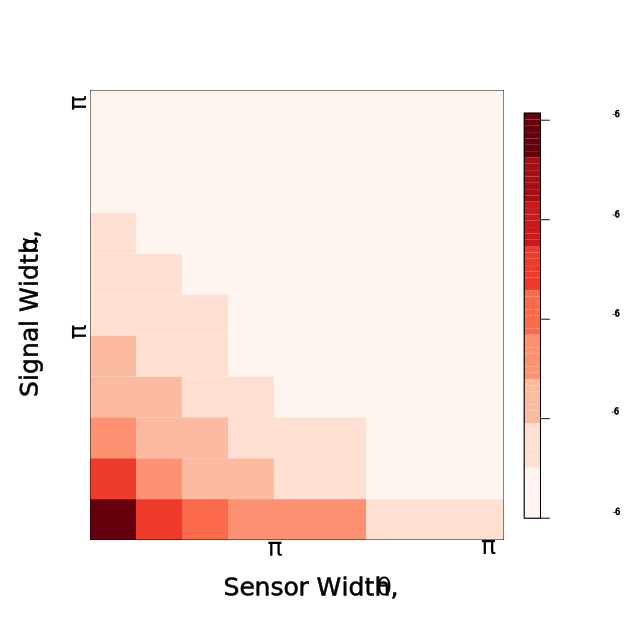
\includegraphics[width=\textwidth]{imgs/ResultStandardDeviation.pdf}
	\caption[gREM precision given a range of sensor and signal widths]{
Simulation model results of the gREM precision given a range of sensor and signal widths, shown by the standard deviation of the error between the estimated and true densities. 
Standard deviations are shown from deep red to pink, representing high to low values between $0.483\times10^{-6}$ to $3.74\times10^{-6}$. 
        } 
	\label{f:StandardDeviation}
\end{figure}


\clearpage
\section{Supplementary Information: Impact of parameter error}




\begin{figure}[h!]
  \centering
{
  \subfloat[label{f:signal}]{
    \includegraphics[width=0.4\textwidth]{imgs/AverageModelBias_callerror.pdf}
  } 
  \subfloat[label{f:sensor}]{
    \includegraphics[width=0.4\textwidth]{imgs/AverageModelBias_cameraerror.pdf}
  } 
    
	\subfloat[label{f:radius}]{
    \includegraphics[width=0.4\textwidth]{imgs/AverageModelBias_radiuserror.pdf}
  }%%
	\subfloat[label{f:speed}]{
    \includegraphics[width=0.4\textwidth]{imgs/AverageModelBias_speederror.pdf}
  }
}%%
\caption[Model sensitivity to error in parameter estimates]{
Model sensitivity (for all gREM submodels) to error in estimates of a) signal width $\alpha$,  b) sensor width $\theta$, c) detection distance $r$ and d) animal movement speed $v$. 
Estimates are -10\% (red), -1\% (orange), 0\% (grey), +1\% (green) and +10\% (blue) of the true parameter value. 
The black dashed line indicates zero error in density estimates. 
The error bars 95\% confidence intervals across all simulations.
}

\label{f:sensitivity}
\end{figure}












\chapter{Colophon}
\label{appendixlabel3}


This thesis was set using \LaTeX, \XeLaTeX\vspace{1mm} and Bib\LaTeX. \vspace{-0.12cm} 
The formatting is defined by the \href{https://github.com/robjstan/latex-phdthesis}{\emph{phdthesis}} class by Robert Stanley.
The TeX Gyre Pagella typeface is used in the main text while {\usefont{T1}{fla}{l}{n} Lato Light} and {\usefont{T1}{fla}{eb}{n} \color[rgb]{0.75,0.75,0.75} Lato Black} are used in the figures.
Chapters \ref{ch:empirical}, \ref{ch:sims1} and \ref{ch:sims2} are entirely reproducible \href{http://yihui.name/knitr/}{\emph{knitr}} documents \cite{knitr}.
Code for the simulations in Chapter \ref{ch:grem} is not combined into a \emph{knitr} document but code for creating figures is.
All code will be made available on Github at \href{https://github.com/timcdlucas/PhDThesis}. %TODO add dois for thesis and MetapopEpi
Plots were created with a combination of \href{www.inkscape.org}{\emph{Inkscape}}, \emph{ggplot2} \cite{ggplot2}, \emph{palettetown} \cite{palettetown}, \emph{ggtree} \cite{ggtree}, \emph{cowplot} \cite{cowplot} and base \emph{R} \cite{R}.
References were handled with \emph{JabRef} \cite{JabRef_software}. 
 % description of document, e.g. type faces, TeX used, TeXmaker, packages and things used for figures. Like a computational details section.
% e.g. http://tex.stackexchange.com/questions/63468/what-is-best-way-to-mention-that-a-document-has-been-typeset-with-tex#63503

 
% You could separate these out into different files if you have
%  particularly large appendices.

% This line manually adds the Bibliography to the table of contents.
% The fact that \include is the last thing before this ensures that it
% is on a clear page, and adding it like this means that it doesn't
% get a chapter or appendix number.
%\addcontentsline{toc}{chapter}{Bibliography}

% Actually generates your bibliography.
\printbibliography 

% All done. \o/
\end{document}
